\documentclass[a4paper,12pt,oneside,hidelinks]{report}

\usepackage[spanish]{babel}
\usepackage[utf8]{inputenc}
\usepackage{lmodern}
\usepackage[usenames, dvipsnames]{color}
\usepackage{graphicx}
\usepackage{enumerate}
\usepackage{multirow}
\usepackage{graphics}
\usepackage{appendix}
\usepackage[nottoc]{tocbibind}

\usepackage{tikz}
\usetikzlibrary{shapes,arrows,positioning,arrows.meta,fit,backgrounds}
\usepackage{pgfplots}
\pgfplotsset{compat=1.18}
\usepackage{subcaption}
\usepackage{amsmath,amsthm,amssymb}
\usepackage[]{placeins,flafter}
\usepackage[none]{hyphenat} \sloppy
\usepackage{xcolor}
\usepackage{adjustbox}
\usepackage{array}
\usepackage{longtable}
\usepackage{tabularx}
\newcolumntype{L}{>{\raggedright\arraybackslash}X}
\newcolumntype{R}{>{\raggedleft\arraybackslash}X}
\usepackage{amssymb}
\newcommand{\real}[1]{#1}
\usepackage{booktabs}
\usepackage{url}
\usepackage[hidelinks]{hyperref}

%	CONFIGURACIÓN DE PÁGINA

\setlength{\paperwidth}{21cm}          % Ancho de página
\setlength{\paperheight}{29,7cm}       % Alto de página
\setlength{\textwidth}{15.5cm}         % Ancho de zona con texto
\setlength{\textheight}{24.6cm}        % Ancho de zona con texto
\setlength{\topmargin}{-1.0cm}         % Margen superior
                                      
\setlength{\oddsidemargin}{0.46cm}     % Margen izquierdo
\setlength{\evensidemargin}{0.46cm}

\usepackage[skip=9pt]{parskip}
\usepackage{enumitem}
\setlist{nosep, topsep=3pt, partopsep=0pt}
\usepackage{titlesec}
\titleformat{\chapter}[display]
  {\normalfont\huge\bfseries}
  {\chaptertitlename\ \thechapter}
  {16pt}
  {\Huge}
\titlespacing*{\chapter}{0pt}{30pt}{10pt}
\titlespacing*{\section}{0pt}{16pt}{4pt}
\titlespacing*{\subsection}{0pt}{12pt}{2pt}
\titlespacing*{\subsubsection}{0pt}{10pt}{2pt}

\usepackage{makeidx}
\makeindex
\index{key}
\newcommand{\myref}[1]{\color{red}\bf(\ref{#1})}

\begin{document}

%%%%%%%%%%%%%%%%%%%%%%%%%%%%%%%%%%%%%%%%%%%%%%%%%%%%%%%%%%%%%%%%%%%%%%%%%%%%%%%%%%
%		PORTADA
%%%%%%%%%%%%%%%%%%%%%%%%%%%%%%%%%%%%%%%%%%%%%%%%%%%%%%%%%%%%%%%%%%%%%%%%%%%%%%%%%%

\begin{titlepage}

\vspace*{-4mm}
\begin{figure}[!h]
  \centering
	
\includegraphics[width=69.62mm]{Imagenes/UnizarLogo}
\end{figure}

\vspace*{17mm}

\fontsize{28pt}{28pt}\selectfont
\begin{center}
\setlength{\fboxsep}{3.4mm}
\adjustbox{minipage=14.4cm,cfbox=blue,center}{\begin{center} Trabajo Fin de Grado \end{center}}
\end{center}

\vspace*{18.7mm}


\fontsize{20pt}{20pt}\selectfont
\begin{center}
Almacenamiento y Análisis Eficiente de Resultados de Simulaciones Hidráulicas mediante TileDB
\end{center}

\vspace*{0cm} 
\baselineskip 36pt
\begin{center}
\fontsize{12pt}{12pt}\selectfont
\center{\rm  Autor}

\vspace*{3.65mm}
\fontsize{18pt}{18pt}\selectfont
\center{Enrique Baldovín Cotela}
\vspace*{1cm}
\baselineskip 36pt
\fontsize{12pt}{12pt}\selectfont
\center{\rm  Director y Codirector}
\vspace*{3.56mm}
\fontsize{14pt}{14pt}\selectfont
\center{Mario Morales Hernández}
\center{Sergio Ilarri Artigas}
\end{center}

\setcounter{footnote}{1}

\vspace*{16.45mm}
\fontsize{12pt}{12pt}\selectfont
\begin{center}
ESCUELA DE INGENIERÍA Y ARQUITECTURA\\
2026\\
\end{center}


\renewcommand{\thefootnote}{\arabic{footnote}}
\pagenumbering{gobble}
\end{titlepage}
\newpage

\title{Almacenamiento y Análisis Eficiente de Resultados de Simulaciones Hidráulicas mediante TileDB}
\author{Enrique Baldovín Cotela}

\baselineskip 19pt
\renewcommand{\labelitemi}{$-$}
\renewcommand{\tablename}{Tabla}
\renewcommand{\bibname}{Bibliografía}
\renewcommand{\appendixname}{Anexos}
\renewcommand{\appendixtocname}{Anexos}
\renewcommand{\appendixpagename}{Anexos}

\pagenumbering{Roman}

\begin{center}
{\Large \bfseries AGRADECIMIENTOS}
\vspace{2.5cm}
\end{center}


% [Rellenar agradecimientos aquí]

\clearpage
\begin{center}
{\Large \bfseries Almacenamiento y Análisis Eficiente de Resultados de Simulaciones Hidráulicas mediante TileDB}

\vspace{1cm}
{\Large \bfseries RESUMEN}

\vspace{1.5cm}
\end{center}


Este trabajo diseña e implementa un sistema de almacenamiento y análisis eficiente para simulaciones hidráulicas de alta resolución. Las simulaciones del simulador Triton generan hasta 235 GB de datos GeoTIFF por escenario; el \textit{pipeline} ETL desarrollado los transforma en un array TileDB sparse con filtro ByteShuffle+ZSTD-9, reduciéndolos a 17,5 GB (reducción del 92,7\,\%, ratio 13,7$\times$) al almacenar exclusivamente las celdas húmedas, que representan solo el $\sim$8,3\,\% del dominio.

El sistema incluye un motor de 24 consultas analíticas en ocho bloques, que cubren desde consultas básicas de calado y velocidad hasta indicadores de inestabilidad hidrodinámica según los criterios de Russo et al.\ y Xia et al., zona de graves daños normativa (Real Decreto 9/2008) y tiempo de evacuación disponible. Un \textit{benchmark} frente a GeoTIFF muestra ventajas de hasta 12,4$\times$ en cinco de seis patrones de acceso, con resultados consistentes sobre cuatro \textit{datasets} independientes. La validación funcional confirma la exactitud de las consultas mediante comparación sistemática con los datos originales.

El sistema se ha aplicado a 56 simulaciones sobre una cuenca de $\sim$78\,000 km$^2$ en el centro de Estados Unidos, y es generalizable a las salidas de cualquier simulador hidráulico 2D con estructura equivalente. La interfaz de usuario es una aplicación web Streamlit con mapas interactivos, comparativa multi-escenario y exportación a GeoTIFF, desplegada en producción sobre un servidor remoto.



\clearpage

\renewcommand{\contentsname}{Índice}
\tableofcontents

%%%%%%%%%%%%%%%%%%%%%%%%%%%%%%%%%%%%%%%%%%%%%%%%%%%%%%%%%%%%%%%%%%%%%%%%%%%%%%%%%%%
%		Capitulos
%%%%%%%%%%%%%%%%%%%%%%%%%%%%%%%%%%%%%%%%%%%%%%%%%%%%%%%%%%%%%%%%%%%%%%%%%%%%%%%%%%%

\chapter{Introducción y motivación}\label{introduccion-y-motivacion}
\pagenumbering{arabic}

Este capítulo presenta el contexto del trabajo y la problemática que lo motiva. La sección~\ref{contexto-y-motivacion} introduce el contexto de aplicación y el objetivo del proyecto; las secciones~\ref{volumen-y-estructura} a~\ref{patrones-de-acceso} analizan las tres dimensiones de la problemática (volumen de datos, formato de almacenamiento y patrones de acceso); y la sección~\ref{oportunidad-sparse} expone la oportunidad técnica que explora el trabajo y la estructura del resto de la memoria.

\section{Contexto y motivación}\label{contexto-y-motivacion}

La necesidad de un almacenamiento eficiente para resultados de simulaciones hidráulicas surge de dos tendencias: el incremento de la resolución de los modelos hidrodinámicos y la demanda de análisis interactivos sobre volúmenes masivos de datos. Las simulaciones 2D de las ecuaciones de Saint-Venant \cite{saintvenant1871}, con formulaciones eficientes \cite{bates2010simple} e implementaciones sobre GPU \cite{morales2021triton}, permiten hoy modelar inundaciones a escala de cuenca con resolución de metros, generando series temporales de rásteres que alcanzan centenares de gigabytes por escenario. Los formatos habituales de salida no están diseñados para consultas analíticas sobre estos volúmenes. Plataformas como Google Earth Engine \cite{gorelick2017earthengine} han demostrado que desplazar el procesamiento al lugar donde residen los datos reduce drásticamente los tiempos de respuesta \cite{bauer2016earthsystem}, pero están orientadas a datos densos (imágenes satelitales) y carecen de soporte nativo para arrays dispersos, donde la mayor parte de las celdas están secas en cada instante.

El contexto de aplicación son las inundaciones fluviales. El simulador Triton \cite{triton} resuelve la propagación del agua sobre una malla regular y produce, para cada variable física y paso temporal, un fichero GeoTIFF (Geographic Tagged Image File Format) \cite{ogc_geotiff}: un formato ráster estándar en SIG (Sistemas de Información Geográfica) que integra los metadatos de georreferenciación en el propio fichero, pero diseñado para el acceso secuencial y no para el análisis de grandes series temporales. Los resultados permiten evaluar la extensión de la mancha de inundación, identificar zonas de riesgo y comparar escenarios. El \hyperref[anexo-c.-contexto-de-las-simulaciones-hidraulicas]{Anexo~C} amplía este contexto para lectores no familiarizados con la modelización hidráulica.

El objetivo principal de este TFG es diseñar e implementar un sistema de almacenamiento y análisis que permita almacenar estos resultados de forma compacta y eficiente, habilitando consultas analíticas rápidas y visualizaciones interactivas sin necesidad de cargar los rásteres completos en memoria. La Figura~\ref{fig:contexto-problema} resume el contraste entre el enfoque original y la solución propuesta: los GeoTIFF organizan los datos por variable y paso temporal (80 ficheros independientes), lo que obliga a lecturas masivas en serie para las consultas multi-temporales, mientras que el proceso ETL (\textit{Extract, Transform, Load}) los convierte en un array TileDB sparse 3D (tiempo, fila, columna) que almacena únicamente las celdas húmedas y responde las mismas consultas mediante una sola operación indexada.

\begin{figure}[ht]
\centering
\begin{tikzpicture}[
    node distance=6mm,
    arrow/.style={-Latex, thick, draw=black!60},
    etlarrow/.style={-Latex, line width=2pt, draw=blue!70!black},
]

%% —— Nodos principales (se definen antes de dibujar) ——
\node[rectangle, draw=gray!70, fill=black!5, rounded corners=3pt, thick,
      minimum width=50mm, minimum height=42mm] (geo) {};

\node[rectangle, draw=orange!80!black, fill=orange!8, rounded corners=3pt, thick,
      minimum width=50mm, minimum height=42mm, right=38mm of geo] (tdb) {};

%% —— Contenido bloque GeoTIFF ——
\node[font=\small\bfseries, above=2mm] at (geo.north) {GeoTIFF (por escenario)};
\foreach \r in {0,1,2,3} {
    \foreach \c in {0,1,2,3,4} {
        \node[rectangle, draw=gray!50, fill=white, minimum width=7mm, minimum height=5mm]
            at ([xshift=(\c-2)*8.5mm+3mm, yshift=(1.5-\r)*7.5mm] geo.center) {};
    }
}
% Etiquetas de variable: misma fórmula vertical que las filas de la rejilla
\foreach \r/\vn in {0/H, 1/QX, 2/QY, 3/MH} {
    \node[font=\tiny, anchor=east] at ([xshift=-19mm, yshift=(1.5-\r)*7.5mm] geo.center) {\vn};
}
\node[font=\tiny, below=3mm] at (geo.south) {4 variables $\times$ 20 pasos $=$ 80 ficheros $\approx$ 235 GB};

%% —— Contenido bloque TileDB ——
\node[font=\small\bfseries, above=2mm] at (tdb.north) {TileDB sparse};
\begin{scope}[shift={(tdb.center)}]
    \draw[fill=orange!15, draw=orange!70!black, thick] (-1.1cm,-0.75cm) rectangle (1.1cm,0.75cm);
    \draw[fill=orange!25, draw=orange!70!black, thick]
        (-1.1cm,0.75cm) -- (-0.75cm,1.1cm) -- (1.45cm,1.1cm) -- (1.1cm,0.75cm) -- cycle;
    \draw[fill=orange!20, draw=orange!70!black, thick]
        (1.1cm,0.75cm) -- (1.45cm,1.1cm) -- (1.45cm,-0.4cm) -- (1.1cm,-0.75cm) -- cycle;
    \node[font=\tiny\itshape] at (0, 0.15cm) {tiempo};
    \node[font=\tiny\itshape] at (0,-0.2cm) {fila $\times$ col};
\end{scope}
\node[font=\tiny, below=3mm] at (tdb.south) {Solo celdas húmedas $\approx$ 17{,}5 GB ($-$93\,\%)};

%% —— Cajas de consulta ——
\node[rectangle, draw=red!60, fill=red!5, rounded corners=2pt, dashed, thick,
      align=center, font=\scriptsize, minimum width=50mm, below=10mm of geo] (qgeo)
    {\textbf{Q7: hora de llegada del frente}\\
     Leer 20 ficheros en secuencia $\to$ varios minutos};

\node[rectangle, draw=green!60!black, fill=green!5, rounded corners=2pt, dashed, thick,
      align=center, font=\scriptsize, minimum width=50mm, below=10mm of tdb] (qtdb)
    {\textbf{Q7: misma consulta}\\
     1 operación sobre el array $\to$ 79{,}5 s};

%% —— Flechas ——
\draw[etlarrow] (geo.east) -- node[above, font=\small\bfseries, text=blue!70!black] {ETL}
                                node[below, font=\scriptsize, text=blue!60] {ingesta + compresión}
               (tdb.west);
\draw[arrow, draw=red!60]        (geo.south)  -- (qgeo.north);
\draw[arrow, draw=green!60!black] (tdb.south) -- (qtdb.north);

\end{tikzpicture}
\caption{Contexto del trabajo: del almacenamiento original en GeoTIFF al array TileDB sparse.}
\label{fig:contexto-problema}
\end{figure}
\FloatBarrier

La problemática de partida combina tres dimensiones que se refuerzan entre sí: un volumen de datos considerable, un formato de almacenamiento no diseñado para análisis y unos patrones de acceso que el formato no cubre con eficiencia.

\section{Volumen y estructura de los datos}\label{volumen-y-estructura}

Cada simulación con el simulador Triton produce 80 ficheros GeoTIFF georreferenciados (4 variables físicas $\times$ 20 pasos temporales), con un tamaño aproximado de 3 GB por fichero y un total cercano a 235 GB por escenario. El dominio espacial está discretizado en una malla regular de 34 200 $\times$ 23 040 píxeles, lo que supone aproximadamente 787 millones de celdas por paso temporal y unas 15 700 millones de celdas en la simulación completa. Procesar este volumen con herramientas convencionales exige cargar cada ráster completo en memoria, lo que requiere alrededor de 3 GB por variable y resulta inviable en estaciones de trabajo con menos de 32 GB de RAM.

\section{Inadecuación del formato GeoTIFF para consultas analíticas}\label{inadecuacion-geotiff}

GeoTIFF \cite{ogc_geotiff} está concebido para el acceso eficiente a un único ráster: no incorpora un motor de consultas, no indexa subconjuntos espaciales o temporales y no permite filtrar por valor sin descomprimir el ráster completo. Operaciones habituales como ``calcular la primera hora en que el agua llega a cada celda'' exigen recorrer y descomprimir los 20 pasos temporales: sobre 235 GB de datos crudos, esto supone tiempos del orden de minutos a horas y, en algunos casos, fallos por agotamiento de memoria.

\section{Patrones de acceso típicos del análisis hidráulico}\label{patrones-de-acceso}

El usuario final no consulta los datos como rásteres aislados, sino como una colección espacio-temporal coherente. Los patrones de acceso más habituales son cinco:

\begin{itemize}
\item \textbf{Consultas en un punto o zona}: Valor de calado en un punto y un instante concretos, o serie temporal completa en un punto.
\item \textbf{Consultas espaciales acotadas}: Estadísticos o mapas sobre una ventana geográfica reducida (por ejemplo, un núcleo urbano de 5$\times$5 km).
\item \textbf{Consultas multi-temporales}: Agregados sobre los 20 pasos temporales completos (hora de llegada del frente, duración total de la inundación, calado máximo por celda).
\item \textbf{Consultas de peligrosidad}: Clasificación de cada celda según criterios combinados de calado y caudal unitario (Russo et al. 2013 \cite{russo2013}).
\item \textbf{Consultas comparativas}: Contraste de métricas entre varios escenarios simulados (por ejemplo, año seco frente a año húmedo).
\end{itemize}

Tres de ellos (espaciales acotados, multi-temporales y peligrosidad) penalizan especialmente la lectura directa de GeoTIFF, y los cinco determinan el diseño de las 24 consultas del motor analítico.

\section{Oportunidad: dominio mayoritariamente seco}\label{oportunidad-sparse}

En una inundación típica solo el $\sim$8,3 \% de las celdas del dominio contiene agua en cada paso temporal ($\sim$65 millones de las $\sim$787 millones totales); el resto son celdas secas sin información útil. Esta característica convierte el almacenamiento disperso (que solo guarda las celdas no nulas y sus coordenadas) en un candidato natural, y constituye la oportunidad técnica que explora este trabajo.

Tras este capítulo introductorio, el capítulo~\ref{descripcion-de-los-datos} describe los datos de entrada; el capítulo~\ref{analisis-de-tecnologias} analiza las tecnologías evaluadas y el funcionamiento de TileDB; el capítulo~\ref{diseno-del-sistema} presenta el diseño del sistema, el proceso ETL y la elección experimental de la configuración de almacenamiento; el capítulo~\ref{herramientas-desarrolladas} las herramientas desarrolladas (motor de consultas, comparativa frente a GeoTIFF y aplicación web); el capítulo~\ref{validacion-del-sistema} la validación y el rendimiento; y el capítulo~\ref{conclusiones-y-trabajo-futuro} las conclusiones. Los Anexos A--E completan la memoria con el catálogo de consultas, las tablas detalladas del \textit{benchmark}, el contexto hidráulico, el proceso ETL detallado y la guía de despliegue.


\chapter{Descripción de los Datos}\label{descripcion-de-los-datos}

Este capítulo describe los datos de entrada del sistema: el simulador hidráulico que los genera, el formato de salida GeoTIFF, las variables físicas almacenadas en cada paso temporal y las características del dominio de simulación.

\section{Simulador Triton}\label{simulador-triton}

Triton \cite{triton} es un simulador hidráulico bidimensional de alto rendimiento desarrollado en el Oak Ridge National Laboratory. Resuelve las ecuaciones de Saint-Venant en lámina libre sobre una malla regular, aprovechando la paralelización masiva en GPU (\textit{Graphics Processing Unit}) para reducir drásticamente los tiempos de cómputo respecto a simuladores tradicionales de CPU. Esta capacidad lo hace adecuado para estudios a gran escala como el de este trabajo, en el que se simulan 56 episodios de crecida sobre una cuenca de $\sim$78\,000 km$^2$ con resolución de 10 m.

Existen otros simuladores hidráulicos 2D ampliamente utilizados, como HEC-RAS \cite{hecras}, IBER \cite{iber} o LISFLOOD-FP \cite{lisflood}. Todos ellos comparten la misma naturaleza de resultados: series temporales de variables físicas organizadas en mallas rásteres regulares. La elección de Triton en este proyecto viene determinada por su uso en el grupo de investigación y por su rendimiento en dominios de alta resolución, pero el problema de almacenamiento y análisis que se aborda no es específico de él. El sistema desarrollado, que comprende la ingesta desde GeoTIFF y el motor de consultas sobre TileDB, es aplicable a las salidas de cualquier simulador que produzca rásters georreferenciados con la misma estructura: los únicos parámetros que cambiarían serían los nombres de las variables y las dimensiones del dominio.

\section{Formato de salida: GeoTIFF}\label{formato-de-salida-geotiff}

GeoTIFF (Geographic Tagged Image File Format) \cite{ogc_geotiff} es el formato más extendido para guardar datos geográficos en forma de cuadrícula (imágenes de satélite, modelos de elevación, mapas de inundación, etc.). Conceptualmente es una matriz bidimensional de valores numéricos en la que cada celda (fila, columna) representa una porción cuadrada del terreno con un valor asociado (por ejemplo, la profundidad del agua en metros). Se diferencia de una imagen convencional (JPG, PNG) en dos aspectos: las celdas guardan magnitudes físicas en lugar de colores y el fichero incluye los metadatos geográficos necesarios para saber qué zona del mundo cubre, qué tamaño tiene cada celda sobre el terreno y en qué sistema de coordenadas está representado.

En este proyecto, cada GeoTIFF contiene la matriz de valores de una variable física (calado, caudal, etc.) en un instante concreto. Triton genera un fichero por cada combinación de variable y paso temporal: cuatro variables (H, QX, QY, MH) por cada uno de los 20 pasos producen 80 ficheros por escenario, que ocupan aproximadamente 235 GB en total. Este formato es muy adecuado para visualizar un mapa concreto en programas como QGIS, pero no está pensado para realizar consultas analíticas sobre toda la serie temporal (motivos detallados en la sección~\ref{inadecuacion-geotiff}), lo que motiva la búsqueda de un sistema de almacenamiento alternativo analizado en las secciones~\ref{bases-de-datos-para-arrays-multidimensionales} y~\ref{justificacion-de-tiledb}.

\section{Variables almacenadas}\label{variables-almacenadas}

Cada paso temporal almacena cuatro variables por celda húmeda (toda celda con calado H $\geq$ 0,01 m), recogidas en la Tabla~\ref{tab:variables}:

\begin{table}[ht]
\centering
\begin{tabularx}{\textwidth}{>{\centering\arraybackslash}p{2cm}L>{\centering\arraybackslash}p{2cm}}
\toprule
\textbf{Variable} & \textbf{Descripción} & \textbf{Unidad} \\
\midrule
H  & Profundidad instantánea del agua & m \\
QX & Caudal unitario en dirección X & m\textsuperscript{2}/s \\
QY & Caudal unitario en dirección Y & m\textsuperscript{2}/s \\
MH & Profundidad máxima acumulada desde el inicio (máximo histórico) & m \\
\bottomrule
\end{tabularx}
\caption{Variables almacenadas por celda y paso temporal.}
\label{tab:variables}
\end{table}

Solo se almacenan celdas con H $\geq$ 0,01 m (umbral de celda húmeda). El módulo del caudal unitario Q\_mod = $\sqrt{QX^2 + QY^2}$ se calcula en tiempo de consulta a partir de QX y QY.

\section{Características del dominio}\label{caracteristicas-del-dominio}

El dominio de simulación cubre una cuenca hidrográfica discretizada en una malla regular de 34 200 $\times$ 23 040 píxeles ($\sim$787 millones de celdas) con resolución espacial de 10 $\times$ 10 m (100 m\textsuperscript{2} por celda). Las características principales se resumen en la Tabla~\ref{tab:dominio}.

Sistema de referencia: EPSG:32614 (UTM zona 14N). El dominio abarca una cuenca de $\sim$342 $\times$ 230 km en el centro-norte de Estados Unidos (Nebraska, Kansas, Iowa y Missouri). Esquina inferior-izquierda: X = 680 000 m, Y = 4 330 000 m.

Resolución temporal: 20 pasos de 6 horas cada uno, cubriendo 120 horas (5 días) de simulación.

Fracción húmeda media: aproximadamente el 8,3 \% de las celdas del dominio presentan agua en cada paso temporal ($\sim$65 millones de celdas de $\sim$787 millones totales). Esta escasez justifica el uso de almacenamiento disperso.

La sección~\ref{analisis-de-tecnologias} justifica la elección de TileDB como tecnología de almacenamiento a partir de las características del problema.


\noindent\begin{minipage}{\textwidth}
\begin{tabularx}{\textwidth}{>{\raggedright\arraybackslash}p{5.5cm}L}
\toprule
\textbf{Parámetro} & \textbf{Valor} \\
\midrule
Resolución espacial & 34\,200 $\times$ 23\,040 píxeles (filas $\times$ columnas) \\
Pasos temporales & 20 (intervalos de 6 h, 120 h totales) \\
Total de celdas & 15\,759\,360\,000 \\
Celdas con agua (H $\geq$ 0,01 m) & 1\,311\,695\,098 ($\sim$8,3 \%) \\
\bottomrule
\end{tabularx}
\captionsetup{hypcap=false}\captionof{table}{Características del dominio de simulación.}
\label{tab:dominio}
\end{minipage}


\chapter{Análisis de Tecnologías}\label{analisis-de-tecnologias}

Antes de comenzar el desarrollo se realizó un análisis de las tecnologías disponibles para almacenar grandes volúmenes de datos ráster espacio-temporales, con el objetivo de seleccionar la más adecuada en términos de eficiencia de almacenamiento, velocidad de consulta y facilidad de integración.

\section{Bases de datos para arrays multidimensionales}\label{bases-de-datos-para-arrays-multidimensionales}

La primera opción considerada fue TileDB \cite{tiledb_github, tiledb_web, tiledb_cmu}, una base de datos de código abierto orientada a arrays N-dimensionales. TileDB soporta tanto arrays densos como dispersos (sparse), compresión pluggable, indexación espacial mediante R-trees y acceso sin servidor, almacenando los datos directamente en el sistema de ficheros.

La segunda opción evaluada fue SciDB \cite{scidb, scidb_docs}, una base de datos nativa para arrays multidimensionales con arquitectura cliente-servidor distribuida: un nodo coordinador reparte el trabajo entre nodos trabajadores y expone los datos mediante lenguajes de consulta propios. Fue descartada por dos motivos: su edición Enterprise (la que ofrece todas las funcionalidades relevantes) es de licencia privativa, lo que limita la reproducibilidad del proyecto; y la necesidad de mantener un servicio en ejecución añade complejidad operativa innecesaria cuando los datos residen en disco local.

La tercera opción considerada fue Rasdaman \cite{rasdaman}, un gestor de bases de datos de arrays N-dimensionales ampliamente utilizado en el ámbito de la observación de la Tierra (es el motor que subyace a algunos servicios de Copernicus). Ofrece un lenguaje de consulta propio (RasQL) y soporta arrays densos y dispersos. Sin embargo, fue descartado por las mismas razones que SciDB: requiere un servidor en ejecución, lo que añade complejidad operativa, y su edición comunitaria presenta limitaciones funcionales respecto a la edición comercial.

También se evaluó PostGIS Raster \cite{postgis_raster}, la extensión de raster del gestor de bases de datos PostgreSQL. Es una tecnología madura y de código abierto, adecuada para análisis de rásteres 2D estáticos con SQL espacial. No obstante, no está diseñada para arrays N-dimensionales: la dimensión temporal requiere \textit{workarounds} (tablas particionadas, columnas adicionales) y carece de soporte nativo para datos dispersos, lo que la hace poco adecuada para series temporales de simulación hidráulica.

Finalmente, se consideraron tres formatos del ecosistema científico fuera del modelo de base de datos:

\begin{itemize}
\item \textbf{HDF5:} Contenedor binario jerárquico ampliamente usado en ciencias físicas. Soporta compresión y \textit{chunks}, pero no implementa indexación dispersa ni motor de consultas integrado: cualquier consulta espacial requiere reimplementar el filtrado en Python.
\item \textbf{NetCDF-4:} Capa de convenciones sobre HDF5 orientada a datos climáticos. Hereda las mismas limitaciones para datos dispersos.
\item \textbf{Zarr:} Variante moderna inspirada en HDF5 pensada para almacenamiento en la nube. Excelente para arrays densos chunked, pero su soporte para datos dispersos es experimental y carece del modelo de fragmentos por escritura incremental que ofrece TileDB.
\end{itemize}

Finalmente se valoró el uso de estructuras de indexación con resolución variable para almacenar mayor detalle en zonas inundadas y menor en terreno seco; esta funcionalidad la cubre TileDB de forma transparente mediante sus R-trees sobre dimensiones dispersas, sin necesidad de implementación adicional.

\section{Justificación de TileDB}\label{justificacion-de-tiledb}

Se eligió TileDB por cuatro motivos:

\begin{enumerate}
\item \textbf{Código abierto (licencia MIT)}: Garantiza la reproducibilidad del proyecto y permite su uso y modificación sin restricciones.
\item \textbf{Modelo sparse nativo}: Encaja de forma natural con el problema, ya que solo el $\sim$8,3 \% del dominio contiene agua en cada paso temporal (media sobre los 20 pasos); almacenar únicamente las celdas húmedas evita procesar el $\sim$92 \% vacío.
\item \textbf{Arquitectura sin servidor}: Los arrays se almacenan directamente en el sistema de ficheros, sin necesidad de mantener un servicio en ejecución, lo que simplifica el despliegue respecto a alternativas como SciDB.
\item \textbf{Integración Python/NumPy}: La API permite operar sobre los datos directamente desde Python sin capa intermedia, lo que facilita la integración con el resto del ecosistema científico.
\end{enumerate}

El resultado del benchmark confirma la elección: los 235 GB originales en GeoTIFF se reducen a 17,5 GB en TileDB sparse con filtro ByteShuffle+ZSTD-9, un ratio de 13,7$\times$ y una reducción del 92,7 \%, manteniendo tiempos de consulta analítica inferiores a 2 segundos para consultas acotadas y \textit{throughput} superior a 800 MB/s en lecturas masivas. La Tabla~\ref{tab:tecnologias} recoge la comparativa completa de tecnologías evaluadas.

La sección~\ref{tecnologia-tiledb} describe TileDB en detalle y sus características relevantes para este proyecto.


\begin{table}[ht]
\centering
\small
\begin{tabularx}{\textwidth}{>{\raggedright\arraybackslash}p{2.0cm}>{\raggedright\arraybackslash}p{2.4cm}L>{\raggedright\arraybackslash}p{1.5cm}>{\raggedright\arraybackslash}p{2.2cm}>{\raggedright\arraybackslash}p{1.5cm}}
\toprule
\textbf{Tecnología} & \textbf{Código abierto} & \textbf{Modelo} & \textbf{Servidor} & \textbf{Disperso nativo} & \textbf{Decisión} \\
\midrule
TileDB & Sí (MIT) & Array disperso/denso & No & Sí & \textbf{Elegida} \\
SciDB & Parcial (Enterprise privativa) & Array N-dimensional & Sí & Limitado & Descartada \\
Rasdaman & Parcial (Ed. comercial) & Array N-dimensional & Sí & Sí & Descartada \\
PostGIS Raster & Sí & Raster 2D sobre SQL & No & No & Descartada \\
HDF5 & Sí & Contenedor jerárquico & No & No & Descartada \\
Zarr & Sí & Array fragmentado & No & Experimental & Descartada \\
NetCDF-4 & Sí & Capa sobre HDF5 & No & No & Descartada \\
\bottomrule
\end{tabularx}
\caption{Tecnologías evaluadas para el almacenamiento del problema.}
\label{tab:tecnologias}
\end{table}


\section{Lenguaje y bibliotecas}\label{lenguaje-y-librerias}

El desarrollo se realizó en Python, lenguaje de referencia en el ámbito científico y geoespacial, con las siguientes bibliotecas principales:

\begin{itemize}
\item \textbf{Rasterio} \cite{rasterio}: Lectura de ficheros GeoTIFF con soporte para lectura por ventanas (windowed read), permitiendo procesar rásteres de varios GB por franjas sin cargar el fichero completo en memoria.
\item \textbf{NumPy} \cite{numpy}: Operaciones vectorizadas sobre los arrays de datos (máscaras, estadísticas, conversión de tipos).
\item \textbf{TileDB Python:} API para crear, escribir y consultar arrays TileDB sparse desde Python.
\item \textbf{Matplotlib:} Visualización de rásteres, escala logarítmica (LogNorm), flechas de flujo (quiver) y panel de cursor interactivo. Se utiliza en el visualizador de escritorio (visualize\_tiledb.py).
\item \textbf{Streamlit} \cite{streamlit}: Framework web para la aplicación interactiva. Folium y Plotly Express se emplean para mapas interactivos y gráficos temporales dentro de la aplicación.
\end{itemize}



\chapter{Diseño del sistema}\label{diseno-del-sistema}

Este capítulo presenta el diseño del sistema desarrollado: la sección~\ref{arquitectura-general} describe la arquitectura en capas, la sección~\ref{arquitectura-del-array-tiledb} el esquema del array TileDB, la sección~\ref{proceso-de-carga-etl-geotiff_to_tiledb_sparse.py} el proceso de ingesta, la sección~\ref{gestion-de-multiples-escenarios-argumento---dataset} la gestión de múltiples escenarios y la sección~\ref{benchmark-de-almacenamiento} la elección experimental de la configuración de almacenamiento.

\section{Arquitectura general}\label{arquitectura-general}

El sistema está compuesto por cuatro capas articuladas en torno al array TileDB sparse como componente central de almacenamiento, tal y como muestra la Figura~\ref{fig:arquitectura}:

\begin{enumerate}
\item \textbf{Ingesta (ETL):} El módulo de ingesta lee los ficheros GeoTIFF generados por Triton, aplica el filtro de celdas húmedas (H $\geq$ 0,01 m) y escribe los datos en TileDB con filtro ByteShuffle+ZSTD-9. La lectura se realiza por franjas de 5\,000 filas para limitar el uso de memoria.
\item \textbf{Almacenamiento:} Array TileDB sparse con dimensiones (time, row, col) y atributos (H, QX, QY, MH). Un fragmento por paso temporal facilita el filtrado temporal eficiente.
\item \textbf{Análisis:} El motor de consultas proporciona 24 funciones que operan directamente sobre el array TileDB sin exportación previa.
\item \textbf{Visualización y exportación:} Un visualizador interactivo, un exportador a GeoTIFF para interoperabilidad SIG y la aplicación web Streamlit con mapas interactivos, comparativa multi-escenario y panel de ayuda.
\end{enumerate}

\begin{figure}[ht]
\centering
\begin{tikzpicture}[
    font=\small\sffamily,
    node distance=10mm,
    source/.style={rectangle, draw=black!70, fill=black!5, minimum height=11mm, minimum width=22mm, align=center, rounded corners=2pt},
    process/.style={rectangle, draw=blue!70!black, fill=blue!10, minimum height=11mm, minimum width=22mm, align=center, rounded corners=2pt, thick},
    storage/.style={cylinder, draw=orange!80!black, fill=orange!15, shape border rotate=90, aspect=0.25, minimum height=14mm, minimum width=26mm, align=center, thick},
    consumer/.style={rectangle, draw=green!50!black, fill=green!10, minimum height=10mm, minimum width=24mm, align=center, rounded corners=2pt},
    ui/.style={rectangle, draw=red!70!black, fill=red!8, minimum height=10mm, minimum width=28mm, align=center, rounded corners=2pt, thick},
    arrow/.style={-Latex, thick, draw=black!60},
]
    \node[source] (geo) {GeoTIFF Triton\\\scriptsize 1 escenario de simulación};
    \node[process, right=14mm of geo] (etl) {ETL\\\scriptsize filtrado y compresión};
    \node[storage, right=14mm of etl] (tdb) {TileDB sparse\\\scriptsize solo celdas húmedas};

    \node[consumer, below=14mm of tdb, xshift=-32mm] (queries) {Motor de consultas\\\scriptsize 24 funciones analíticas};
    \node[consumer, below=14mm of tdb, xshift=4mm] (viz) {Visualizador};
    \node[consumer, below=14mm of tdb, xshift=40mm] (exp) {Exportador GeoTIFF};

    \node[ui, below=12mm of viz] (app) {Aplicación web Streamlit};

    \draw[arrow] (geo) -- (etl);
    \draw[arrow] (etl) -- (tdb);
    \draw[arrow] (tdb.south) -- ++(0,-3mm) -| (queries.north);
    \draw[arrow] (tdb.south) -- ++(0,-3mm) -| (viz.north);
    \draw[arrow] (tdb.south) -- ++(0,-3mm) -| (exp.north);
    \draw[arrow] (queries.south) -- (app.north);
\end{tikzpicture}
\caption{Arquitectura del sistema en cuatro capas en torno al array TileDB sparse.}
\label{fig:arquitectura}
\end{figure}

\section{Arquitectura del array TileDB}\label{arquitectura-del-array-tiledb}

El array disperso se define con tres dimensiones y cuatro atributos, tal y como se muestra en la Tabla~\ref{tab:array-schema}. Las dimensiones (\texttt{time}, \texttt{row}, \texttt{col}) indexan cada celda húmeda dentro del cubo espacio-temporal, y los cuatro atributos almacenan los valores físicos de esa celda, de modo que una sola consulta puede recuperar cualquier combinación de variables sobre cualquier rango de tiempo y espacio.

\begin{table}[ht]
\centering
\begin{tabularx}{\textwidth}{>{\raggedright\arraybackslash}p{3cm}>{\raggedright\arraybackslash}p{2cm}L}
\toprule
\textbf{Elemento} & \textbf{Tipo} & \textbf{Detalles} \\
\midrule
Dimensión time & int32 & Índice del paso temporal (0--19) \\
Dimensión row & int32 & Fila del ráster (0--34\,199) \\
Dimensión col & int32 & Columna del ráster (0--23\,039) \\
\addlinespace[4pt]
Atributo H & float32 & Profundidad instantánea \\
Atributo QX & float32 & Caudal unitario X \\
Atributo QY & float32 & Caudal unitario Y \\
Atributo MH & float32 & Profundidad máxima histórica \\
\bottomrule
\end{tabularx}
\caption{Dimensiones y atributos del array TileDB sparse.}
\label{tab:array-schema}
\end{table}

La Figura~\ref{fig:tiledb-estructura} ilustra cómo TileDB organiza físicamente estos datos \cite{tiledb_indexing, tiledb_datalayout}: 20 fragmentos independientes (uno por paso temporal) almacenan únicamente las coordenadas y valores de las celdas húmedas, con los cuatro atributos codificados juntos mediante ByteShuffle+ZSTD-9. Cada celda húmeda guarda sus tres coordenadas enteras y los cuatro valores float32; las celdas secas ($\sim$92 \% del dominio) no se almacenan, y esta combinación es la que reduce los $\sim$235 GB originales a $\sim$17,5 GB.

\begin{figure}[ht]
\centering
\begin{tikzpicture}[x=0.9cm, y=0.9cm, font=\small\sffamily]

  %% ── Parámetros (evitar \cs y \rs que son palabras reservadas TeX)
  \pgfmathsetmacro{\FW}{5.0}    % ancho cara frontal
  \pgfmathsetmacro{\FH}{3.2}    % alto cara frontal
  \pgfmathsetmacro{\OX}{0.40}   % offset oblicuo X
  \pgfmathsetmacro{\OY}{0.30}   % offset oblicuo Y
  \pgfmathsetmacro{\CW}{0.48}   % ancho celda mini-grid
  \pgfmathsetmacro{\CH}{0.44}   % alto celda mini-grid

  %% ── Stack de 7 fragmentos (de atrás a delante) ──────────────────
  \foreach \k in {6,5,4,3,2,1,0} {
    \pgfmathsetmacro{\DX}{\k*\OX}
    \pgfmathsetmacro{\DY}{\k*\OY}
    % Cara superior
    \fill[blue!15, draw=blue!28, line width=0.3pt]
      (\DX,\DY+\FH) -- (\DX+\OX,\DY+\FH+\OY)
      -- (\DX+\FW+\OX,\DY+\FH+\OY) -- (\DX+\FW,\DY+\FH) -- cycle;
    % Cara lateral derecha
    \fill[blue!24, draw=blue!28, line width=0.3pt]
      (\DX+\FW,\DY) -- (\DX+\FW+\OX,\DY+\OY)
      -- (\DX+\FW+\OX,\DY+\FH+\OY) -- (\DX+\FW,\DY+\FH) -- cycle;
    % Cara frontal
    \fill[blue!7, draw=blue!35, line width=0.4pt]
      (\DX,\DY) rectangle (\DX+\FW,\DY+\FH);
  }

  %% ── Mini-grid disperso en el fragmento frontal (t_0) ────────────
  % Celdas secas: 10 col x 7 filas = 70 celdas
  \foreach \ci in {0,...,9} {
    \foreach \ri in {0,...,6} {
      \pgfmathsetmacro{\CX}{\ci*\CW + 0.03}
      \pgfmathsetmacro{\CY}{\ri*\CH + 0.03}
      \pgfmathsetmacro{\CXE}{\ci*\CW + \CW - 0.03}
      \pgfmathsetmacro{\CYE}{\ri*\CH + \CH - 0.03}
      \fill[gray!16] (\CX,\CY) rectangle (\CXE,\CYE);
    }
  }
  % Celdas húmedas (~8 %): 6 de 70
  \foreach \ci/\ri in {1/1, 2/3, 4/5, 5/2, 7/4, 8/1, 3/0, 6/5, 0/4, 9/2} {
    \pgfmathsetmacro{\CX}{\ci*\CW + 0.03}
    \pgfmathsetmacro{\CY}{\ri*\CH + 0.03}
    \pgfmathsetmacro{\CXE}{\ci*\CW + \CW - 0.03}
    \pgfmathsetmacro{\CYE}{\ri*\CH + \CH - 0.03}
    \fill[blue!58] (\CX,\CY) rectangle (\CXE,\CYE);
  }

  %% ── Etiquetas de pasos temporales en la cara lateral ────────────
  \foreach \k/\tlabel in {4/$t_{16}$} {
    \pgfmathsetmacro{\DX}{\k*\OX}
    \pgfmathsetmacro{\DY}{\k*\OY}
    \node[blue!50!black, font=\tiny, anchor=west]
      at (\DX+\FW+\OX+0.05, \DY+\FH/2) {\tlabel};
  }
  % t_19 en el fragmento más lejano
  \pgfmathsetmacro{\DXB}{6*\OX}
  \pgfmathsetmacro{\DYB}{6*\OY}
  \node[blue!45!black, font=\tiny, anchor=west]
    at (\DXB+\FW+\OX+0.05, \DYB+\FH/2) {$t_{19}$};
  % "..."
  \pgfmathsetmacro{\DXM}{3.5*\OX}
  \pgfmathsetmacro{\DYM}{3.5*\OY}
  \node[gray!55, font=\normalsize\bfseries]
    at (\DXM+\FW+\OX+0.2, \DYM+\FH/2) {$\cdots$};

  %% ── Ejes ─────────────────────────────────────────────────────────
  % col →
  \draw[-{latex}, gray!55, thick] (0,-0.5) -- (\FW+0.3,-0.5);
  \node[gray!55, font=\scriptsize, below=2pt] at (\FW/2,-0.5)
    {columna \enspace (0\,–\,23\,039)};
  % row ↑
  \draw[-{latex}, gray!55, thick] (-0.45,0) -- (-0.45,\FH+0.2);
  \node[gray!55, font=\scriptsize, rotate=90, above=2pt] at (-0.45,\FH/2)
    {fila \enspace (0\,–\,34\,199)};
  % tiempo ↗
  \pgfmathsetmacro{\TARX}{6*\OX+0.3}
  \pgfmathsetmacro{\TARY}{6*\OY+0.3}
  \draw[-{latex}, blue!50!black, thick] (0,\FH+0.1) -- ++(\TARX,\TARY);
  \node[blue!55!black, font=\scriptsize, rotate=37, above=2pt]
    at (2.0, \FH+0.8) {tiempo (20 fragmentos)};

  %% ── Leyenda (debajo del stack, fuera del área de texto) ─────────
  \pgfmathsetmacro{\LY}{-1.75}
  \fill[blue!58] (0.5,\LY+0.08) rectangle (0.85,\LY+0.38);
  \node[right, font=\tiny] at (0.9,\LY+0.22) {celda h\'{u}meda ($\sim$8\,\%)};
  \fill[gray!16, draw=gray!35, line width=0.3pt]
    (4.2,\LY+0.08) rectangle (4.55,\LY+0.38);
  \node[right, font=\tiny] at (4.6,\LY+0.22) {celda seca (no almacenada)};

  %% ── Cuadro «Estructura por celda» ────────────────────────────────
  \pgfmathsetmacro{\BX}{8.6}
  \pgfmathsetmacro{\BY}{-0.5}
  \pgfmathsetmacro{\BW}{4.8}

  % Cabecera
  \fill[blue!40!black, rounded corners=3pt]
    (\BX,\BY+4.5) rectangle (\BX+\BW,\BY+4.95);
  \node[white, font=\scriptsize\bfseries] at (\BX+\BW/2,\BY+4.72)
    {Estructura por celda};

  % Marco
  \draw[blue!30!black, rounded corners=3pt, thick, fill=blue!3]
    (\BX,\BY) rectangle (\BX+\BW,\BY+4.5);

  % COORDENADAS
  \node[blue!50!black, font=\tiny\bfseries, anchor=west]
    at (\BX+0.12,\BY+4.25) {COORDENADAS};
  \draw[gray!25] (\BX+0.1,\BY+4.08) -- (\BX+\BW-0.1,\BY+4.08);
  \node[font=\tiny, anchor=west] at (\BX+0.15,\BY+3.80) {\texttt{time}};
  \node[font=\tiny, gray!55, anchor=east] at (\BX+\BW-0.1,\BY+3.80) {int32, 0–19};
  \node[font=\tiny, anchor=west] at (\BX+0.15,\BY+3.42) {\texttt{row}};
  \node[font=\tiny, gray!55, anchor=east] at (\BX+\BW-0.1,\BY+3.42) {int32, 0–34\,199};
  \node[font=\tiny, anchor=west] at (\BX+0.15,\BY+3.04) {\texttt{col}};
  \node[font=\tiny, gray!55, anchor=east] at (\BX+\BW-0.1,\BY+3.04) {int32, 0–23\,039};

  % Separador
  \draw[gray!25] (\BX+0.1,\BY+2.78) -- (\BX+\BW-0.1,\BY+2.78);

  % ATRIBUTOS
  \node[orange!60!black, font=\tiny\bfseries, anchor=west]
    at (\BX+0.12,\BY+2.55) {ATRIBUTOS \enspace float32};
  \draw[gray!25] (\BX+0.1,\BY+2.38) -- (\BX+\BW-0.1,\BY+2.38);

  \node[font=\tiny, anchor=west] at (\BX+0.15,\BY+2.12)
    {\texttt{H} \enspace calado instantáneo (m)};
  \node[font=\tiny, anchor=west] at (\BX+0.15,\BY+1.72)
    {\texttt{QX} \enspace caudal unitario X (m²/s)};
  \node[font=\tiny, anchor=west] at (\BX+0.15,\BY+1.32)
    {\texttt{QY} \enspace caudal unitario Y (m²/s)};
  \node[font=\tiny, anchor=west] at (\BX+0.15,\BY+0.92)
    {\texttt{MH} \enspace calado máximo histórico (m)};

  % Separador
  \draw[gray!25] (\BX+0.1,\BY+0.66) -- (\BX+\BW-0.1,\BY+0.66);

  % Compresión y tamaño
  \node[orange!55!black, font=\tiny, align=center]
    at (\BX+\BW/2,\BY+0.43) {ByteShuffle + ZSTD-9};
  \node[gray!55, font=\tiny, align=center]
    at (\BX+\BW/2,\BY+0.18) {$\sim$17,5 GB por escenario};

  %% ── Flecha array → cuadro ────────────────────────────────────────
  \draw[-{latex}, blue!35!black, thick, dashed]
    (\FW+0.12, \FH/2) to[out=5, in=175] (\BX-0.1, \BY+2.5);

\end{tikzpicture}
\caption{Estructura interna del array TileDB sparse: fragmentos por paso temporal (izquierda) y contenido de cada celda húmeda (derecha).}
\label{fig:tiledb-estructura}
\end{figure}

\FloatBarrier
\section{Proceso de carga ETL (geotiff\_to\_tiledb\_sparse.py)}\label{proceso-de-carga-etl-geotiff_to_tiledb_sparse.py}

Se ha creado un script en Python que carga los GeoTIFF de un escenario a TileDB. Para cada paso temporal, el cargador abre los 4 ficheros GeoTIFF con rasterio y los lee en paralelo (\texttt{ThreadPoolExecutor}) por franjas de 5\,000 filas para limitar la memoria (pico $\approx$ 1,8 GB), aplica la máscara de celdas húmedas (H $\geq$ 0,01 m) y realiza una única escritura en TileDB, generando un fragmento por paso. Al finalizar verifica la integridad del array mediante muestreo aleatorio contra los GeoTIFF originales. El diagrama de flujo completo (Figura~\ref{fig:etl-flow}) y los parámetros del proceso se recogen en el \hyperref[anexo-d.-proceso-de-ingesta-etl-detallado]{Anexo~D}.

\FloatBarrier
\section{Gestión de múltiples escenarios}\label{gestion-de-multiples-escenarios-argumento---dataset}

El sistema procesa y almacena múltiples escenarios de forma independiente. Cada escenario ocupa su propio array TileDB y se identifica mediante un alias corto (datos1, datos2, \ldots) que \texttt{config.py} traduce al nombre real del directorio de salida de Triton; el módulo de ingesta acepta el argumento \texttt{-\/-dataset} para seleccionar el escenario, y dos variables de entorno controlan las rutas de datos (detalladas, junto con la estructura de directorios, en el \hyperref[anexo-e.-guia-de-despliegue]{Anexo~E}).

La aplicación web descubre automáticamente los \textit{datasets} disponibles inspeccionando el directorio de arrays: cualquier subdirectorio con un array TileDB válido aparece en el selector de la interfaz, con la fecha de inicio extraída del nombre del directorio. Añadir un nuevo escenario consiste únicamente en ejecutar el ETL con el alias correspondiente.

\section{Elección de la configuración de almacenamiento}\label{benchmark-de-almacenamiento}

La última decisión de diseño es la configuración de almacenamiento del array, determinada mediante un \textit{benchmark} sistemático ejecutado sobre los datos reales del dominio de simulación. Se evaluaron cinco grupos de parámetros de forma independiente (G1--G5: filtros de compresión, tamaño de \textit{tile}, tipo de dato, organización temporal y estructura de atributos) y se adoptó la configuración definitiva que se aplica a los 56 conjuntos de datos procesados.

El ahorro de espacio proviene principalmente del almacenamiento disperso (solo el $\sim$8,3 \% del dominio está inundado), no de la compresión en sí; las métricas del array con la configuración inicial (ZSTD-1) se recogen en la Tabla~\ref{tab:metricas-tdb} del \hyperref[anexo-b.-tablas-de-resultados-completas]{Anexo~B}. Para cuantificar el impacto de la compresión se diseñó un \textit{benchmark} con cinco dimensiones de experimento, ejecutado sobre los datos reales del paso temporal 16\_00 (64,3 millones de celdas húmedas, en torno al $\sim$8,3 \% de los 787 millones del paso).

\subsection{Entorno y metodología experimental}\label{entorno-y-metodologia-experimental}\label{hardware-y-software}

Todos los experimentos se realizaron en la misma máquina para garantizar la comparabilidad de los resultados. Hardware: procesador AMD Ryzen 9 7900X (12 núcleos / 24 hilos, 4,7--5,6 GHz), 32 GB de RAM DDR5 a 5\,200 MT/s, almacenamiento SSD (\textit{Solid-State Drive}) NVMe PCIe Gen4 de 2 TB. Software: Windows 11 Pro con subsistema WSL2 (Windows Subsystem for Linux~2, Ubuntu 24.04 LTS, kernel 6.6), Python 3.12.3, TileDB 0.36.1, NumPy 2.4.4, rasterio 1.5.0, Streamlit 1.36.

\label{protocolo-de-medicion}Cada caso de prueba sigue el mismo protocolo de medición. Los \textit{benchmarks} de patrones de acceso se ejecutan tres veces y se reporta la mediana; el de filtros de compresión usa 200 repeticiones sobre una región fija de 5\,000$\times$5\,000 celdas. Antes de cada serie se libera la caché de páginas del sistema operativo para medir el tiempo en frío; las repeticiones siguientes miden el tiempo en caché caliente, que es el valor reportado en las tablas. La RAM pico se mide con \texttt{tracemalloc} (los matices de esta medición y el cálculo del \textit{throughput} se detallan en el \hyperref[anexo-b.-tablas-de-resultados-completas]{Anexo~B}). Todos los scripts están versionados en el repositorio y son reejecutables con un único argumento; los tiempos absolutos dependen del hardware, pero los factores relativos entre TileDB y GeoTIFF son directamente comparables.

\subsection{Resultado final: configuración definitiva}\label{resultado-final-configuracion-definitiva}

A partir de los resultados del \textit{benchmark} se generaron los 56 arrays definitivos (triton\_results/datos1--datos56) con el filtro ByteShuffle + ZSTD-9, manteniendo el resto de parámetros de producción (float32, tile 256$\times$256, array 3D con 1 fragmento por paso, multi-atributo). La Tabla~\ref{tab:benchmark-resumen} resume las comparativas realizadas y la decisión adoptada en cada grupo; los resultados detallados se recogen en el \hyperref[anexo-b.-tablas-de-resultados-completas]{Anexo~B}.

\begin{table}[ht]
\centering
\small
\begin{tabularx}{\textwidth}{>{\raggedright\arraybackslash}p{4.6cm}>{\raggedright\arraybackslash}p{2.9cm}L}
\toprule
\textbf{Grupo (alternativas comparadas)} & \textbf{Elegida} & \textbf{Motivo principal} \\
\midrule
G1. Filtros (ZSTD 1/3/5/9, ByteShuffle+ZSTD, BitShuffle+ZSTD) & ByteShuffle+ ZSTD-9 & ByteShuffle reordena los bytes de los float32 antes de comprimir: $-$16 \% frente a sin compresión; velocidad de lectura equivalente entre variantes \\
\addlinespace[3pt]
G2. Tile espacial (256, 512, 1\,024) & 256$\times$256 & Diferencias despreciables con datos dispersos \\
\addlinespace[3pt]
G3. Tipo de dato (float64, float32, float16) & float32 & float64 ocupa +9,4 \%; float16 no soportado \\
\addlinespace[3pt]
G4. Estructura temporal (tile\_t=1 vs 4; 2D vs 3D) & Array 3D, 1 frag./paso & Confinar cada tile a un paso comprime $-$19 \% y permite filtrado temporal sin consolidación \\
\addlinespace[3pt]
G5. Atributos (1 array multi-atributo vs 4 arrays) & 1 array, 4 atributos & Arrays separados: +14,9 \% en disco y 2,2$\times$ más lentos en lectura conjunta \\
\bottomrule
\end{tabularx}
\caption{Resumen del \textit{benchmark} de almacenamiento por grupos de parámetros.}
\label{tab:benchmark-resumen}
\end{table}


\begin{table}[ht]
\centering
\begin{tabularx}{\textwidth}{>{\raggedright\arraybackslash}p{5.5cm}LL}
\toprule
& \textbf{Configuración inicial (ZSTD-1)} & \textbf{Configuración final (ByteShuffle + ZSTD-9)} \\
\midrule
Tamaño total (20 pasos) & 19\,327 MB & 17\,611 MB \\
Ahorro respecto a configuración inicial & --- & \textbf{$-$1\,716 MB ($-$8,9\,\%)} \\
Mediana lectura región & $\sim$0,158 s & $\sim$0,196 s (similar) \\
Tiempo de carga & $\sim$454 s & $\sim$477 s \\
\bottomrule
\end{tabularx}
\caption{Comparativa entre la configuración inicial y la configuración final del array TileDB.}
\label{tab:configuracion-final}
\end{table}


La configuración final ocupa 1\,716 MB menos (-8,9 \%) con tiempos de lectura equivalentes. El incremento de tiempo de carga (+22 s sobre 477 s totales) es asumible dado que la ingesta es un proceso puntual frente a la consulta continua de los datos. Las herramientas construidas sobre esta configuración se presentan en el capítulo~\ref{herramientas-desarrolladas}, y su validación y rendimiento en el capítulo~\ref{validacion-del-sistema}.


\chapter{Benchmark de Almacenamiento}\label{benchmark-de-almacenamiento}

La Tabla~\ref{tab:metricas-tdb} resume las métricas globales del array TileDB sparse con la configuración inicial (ZSTD-1) sobre datos1, previa al \textit{benchmark} de configuraciones de compresión.

\begin{table}[ht]
\centering
\begin{tabularx}{\textwidth}{>{\raggedright\arraybackslash}p{9.5cm}L}
\toprule
\textbf{Métrica} & \textbf{Valor} \\
\midrule
Pasos temporales & 20 \\
Resolución ráster & 34 200 $\times$ 23 040 px \\
Variables & H, QX, QY, MH \\
Celdas totales del dominio & 15 759 360 000 \\
Celdas almacenadas en TileDB & 1 311 695 098 \\
\% del dominio con agua & 8,3 \% \\
\addlinespace[6pt]
Ficheros GeoTIFF originales & 235 GB \\
TileDB sparse (ZSTD-1) & 19 GB \\
Espacio ahorrado & 216 GB (91,9 \%) \\
Ratio de compresión & 12,4$\times$ \\
\addlinespace[6pt]
Bytes/celda sin comprimir (4 vars $\times$ float32) & 16 B \\
Bytes/celda en TileDB & 15,6 B \\
Tiempo de carga (20 pasos) & 454 s ($\sim$7,5 min) \\
\bottomrule
\end{tabularx}
\caption{Métricas globales del array TileDB sparse con configuración inicial ZSTD-1 (datos1). La configuración definitiva tras el benchmark se recoge en la Tabla~\ref{tab:configuracion-final}.}
\label{tab:metricas-tdb}
\end{table}


El ahorro de espacio proviene principalmente del almacenamiento disperso (solo el $\sim$8,3 \% del dominio está inundado), no de la compresión en sí. Para cuantificar el impacto de distintas configuraciones de compresión se diseñó un \textit{benchmark} exhaustivo con cinco dimensiones de experimento, ejecutado sobre los datos reales del paso temporal 16\_00 (64,3 millones de celdas húmedas). Las lecturas se midieron sobre una región fija de 5 000$\times$5 000 celdas con 200 repeticiones para obtener resultados estadísticamente robustos.

\section{Entorno y metodología experimental}\label{entorno-y-metodologia-experimental}

Todos los experimentos se realizaron en la misma máquina para garantizar la comparabilidad de los resultados.

\subsection{Hardware y software}\label{hardware-y-software}

Hardware: procesador AMD Ryzen 9 7900X (12 núcleos / 24 hilos, 4,7--5,6 GHz), 32 GB de RAM DDR5 a 5200 MT/s, almacenamiento SSD (\textit{Solid-State Drive}) NVMe PCIe Gen4 de 2 TB.

Software: Windows 11 Pro con subsistema WSL2 (Ubuntu 24.04 LTS, kernel 6.6), Python 3.12.3, TileDB 0.36.1, NumPy 2.4.4, rasterio 1.5.0, Streamlit 1.36.

\subsection{Protocolo de medición}\label{protocolo-de-medicion}

Cada caso de prueba se ejecuta siguiendo el mismo protocolo:

\begin{itemize}
\item \textbf{Repeticiones.} Los \textit{benchmarks} de patrones de acceso (5 patrones en \texttt{benchmark\_queries.py} y 6 casos en \texttt{benchmark\_vs\_geotiff.py}) se ejecutan tres veces consecutivas y se reporta la mediana. Para el benchmark de filtros de compresión, en el que la dispersión es relevante para discriminar configuraciones similares, se ejecutaron 200 repeticiones sobre una región fija de 5 000$\times$5 000 celdas y se reporta mediana y desviación típica.

\item \textbf{Caché fría frente a caché caliente.} Antes de cada serie de repeticiones la caché de páginas del sistema operativo se libera con \texttt{sync \&\& echo 3 > /proc/sys/vm/drop\_caches} para medir el tiempo en frío de la primera lectura. Las repeticiones segunda y tercera se ejecutan sin liberar caché y miden el tiempo en caché caliente, que es el valor reportado en las tablas comparativas. La diferencia entre ambos tiempos cuantifica la sensibilidad de cada motor (TileDB y GeoTIFF) al estado de la caché del sistema operativo.

\item \textbf{Medición de RAM.} El consumo de memoria se mide con la biblioteca estándar \texttt{tracemalloc} de Python, registrando el pico de asignación entre el inicio y el fin de cada operación. Esta herramienta captura las asignaciones realizadas a través del asignador de Python, lo que incluye los arrays de NumPy devueltos por TileDB y rasterio. Los buffers internos asignados directamente en C (por ejemplo, los tiles descomprimidos por TileDB o las bandas leídas por GDAL antes de pasar a NumPy) no son visibles para \texttt{tracemalloc}, por lo que los valores reportados deben interpretarse como una cota inferior del consumo total del proceso, no como su valor exacto.

\item \textbf{Throughput.} Se calcula como $\text{bytes\_descomprimidos} / \text{tiempo\_caliente}$, donde \texttt{bytes\_descomprimidos} es el tamaño en memoria de los datos devueltos al cliente: $N_{\text{celdas}} \times N_{\text{variables}} \times 4$ bytes para float32. En TileDB sparse $N_{\text{celdas}}$ corresponde al número de celdas húmedas en la región consultada; en GeoTIFF es el tamaño completo de la ventana leída, incluyendo celdas secas.

\item \textbf{Reproducibilidad.} Todos los scripts de \textit{benchmark} están versionados en el directorio \texttt{spillway/} del proyecto y son reejecutables con un único argumento (\texttt{--dataset}). Los tiempos absolutos dependen del hardware; los factores relativos entre TileDB y GeoTIFF son los resultados directamente comparables.
\end{itemize}

\section{Resultado final: configuración definitiva}\label{resultado-final-configuracion-definitiva}

A partir de los resultados del \textit{benchmark} se generaron los 56 arrays definitivos (triton\_results/datos1--datos56) con el filtro ByteShuffle + ZSTD-9, manteniendo el resto de parámetros de producción (float32, tile 256$\times$256, array 3D con 1 fragmento por paso, multi-atributo).

El \textit{benchmark} evalúa cinco grupos de parámetros de forma independiente (G1--G5). La Tabla~\ref{tab:benchmark-resumen} resume las comparativas realizadas y la decisión adoptada en cada caso. Los resultados detallados se recogen en el Anexo B.

\begin{center}
\begin{tabularx}{\textwidth}{>{\raggedright\arraybackslash}p{3cm}>{\raggedright\arraybackslash}p{3.8cm}L>{\raggedright\arraybackslash}p{2.8cm}}
\toprule
\textbf{Grupo} & \textbf{Comparación} & \textbf{Resultado} & \textbf{Configuración elegida} \\
\midrule
G1.\\ Filtros & ZSTD puro (niveles 1, 3, 5, 9), ByteShuffle+ZSTD, BitShuffle+ZSTD & \textbullet~ByteShuffle+ZSTD-9: menor tamaño ($-$8,9 \% vs ZSTD-1). \newline \textbullet~Lectura similar entre variantes shuffle. & ByteShuffle+ZSTD-9 \\
G2.\\ Tile espacial & Tiles 256$\times$256, 512$\times$512 y 1\,024$\times$1\,024 celdas & \textbullet~Diferencias despreciables en tamaño y velocidad con datos dispersos. & 256$\times$256 \\
G3.\\ Tipo de dato & float64 (nativo GeoTIFF), float32, float16 & \textbullet~float16 no soportado. \newline \textbullet~float64: +9,4 \% sobre float32. \newline \textbullet~float32: equilibrio tamaño/precisión. & float32 \\
G4.\\ Estructura temporal & tile\_t=1 vs tile\_t=4; array 2D vs 3D & \textbullet~tile\_t=1: $-$19 \% frente a tile\_t=4. \newline \textbullet~1 fragmento/paso facilita el filtrado temporal. & Array 3D, 1 frag./paso \\
G5.\\ Atributos & 1 array multi-atributo vs 4 arrays independientes & \textbullet~Arrays separados: +14,9 \% en disco y 2,2$\times$ más lentos en lectura conjunta. & 1 array, 4 atributos \\
\bottomrule
\end{tabularx}
\captionsetup{hypcap=false}\captionof{table}{Resumen del benchmark de almacenamiento por grupos de parámetros.}
\label{tab:benchmark-resumen}
\end{center}


\begin{table}[ht]
\centering
\begin{tabularx}{\textwidth}{>{\raggedright\arraybackslash}p{5.5cm}LL}
\toprule
& \textbf{Configuración inicial (ZSTD-1)} & \textbf{Configuración final (ByteShuffle + ZSTD-9)} \\
\midrule
Tamaño total (20 pasos) & 19\,327 MB & 17\,613 MB \\
Ahorro respecto a configuración inicial & --- & \textbf{$-$1\,714 MB ($-$8,9\,\%)} \\
Mediana lectura región & $\sim$0,158 s & $\sim$0,196 s (similar) \\
Tiempo de carga & $\sim$454 s & $\sim$477 s \\
\bottomrule
\end{tabularx}
\caption{Comparativa entre la configuración inicial y la configuración final del array TileDB.}
\label{tab:configuracion-final}
\end{table}


La configuración final ocupa 1 714 MB menos (-8,9 \%) con tiempos de lectura equivalentes. El incremento de tiempo de carga (+22 s sobre 477 s totales) es asumible dado que la ingesta es un proceso puntual frente a la consulta continua de los datos.

Las herramientas de análisis y visualización construidas sobre el sistema se presentan en la sección~\ref{herramientas-desarrolladas}.

\section{Evaluación de rendimiento de las consultas analíticas}\label{evaluacion-rendimiento-consultas}

Para cuantificar el coste real de las consultas sobre el sistema definitivo, se midió el tiempo de ejecución de las principales funciones del motor analítico sobre \texttt{datos29}, el \textit{dataset} más voluminoso disponible (21 GB, 20 fragmentos, dominio de 34\,200\,$\times$\,23\,040 px). Las mediciones se realizaron en la máquina de desarrollo descrita en la Sección~\ref{hardware-y-software} (AMD Ryzen 9 7900X, 32 GB DDR5, SSD NVMe PCIe Gen4). Cada consulta se ejecutó una sola vez sobre caché fría, que es la condición real de uso: el usuario lanza una consulta bajo demanda sin garantía de que los datos estén en caché.

Las consultas se agrupan en tres categorías según su patrón de acceso a TileDB:

\begin{itemize}
\item \textbf{Instantáneas.} Acceden a un único fragmento (un paso temporal). Su coste es proporcional al número de celdas húmedas en ese instante.
\item \textbf{Multi-paso.} Recorren los 20 fragmentos secuencialmente acumulando un escalar o vector por paso. Son el grupo de mayor volumen de E/S.
\item \textbf{Acumuladas por píxel.} También recorren los 20 fragmentos, pero actualizan en cada paso un \textit{grid} de tamaño fijo $n_r \times n_c$ (sección~\ref{motor-de-consultas-analiticas}). Son las más costosas porque combinan E/S intensiva con escrituras dispersas en memoria.
\end{itemize}

La Figura~\ref{fig:patrones-acceso} ilustra estos tres patrones sobre el array TileDB. La Tabla~\ref{tab:benchmark-consultas} recoge los tiempos para el dominio completo y para un subdominio central del 50\,\% en cada eje (25\,\% del área total), que ilustra la ganancia cuando el usuario restringe la consulta a un área de interés mediante un \textit{bounding box}.

\begin{figure}[ht]
\centering
\begin{tikzpicture}[x=0.62cm, y=0.62cm, font=\small\sffamily]
  %% Tres paneles horizontales (tiempo × espacio), W=5 H=3 unidades
  %% Separación entre paneles: 1.5 unidades

  %% ---- Panel 1: Instantánea ----
  \fill[gray!10] (0,0) rectangle (5,3);
  \draw[gray!50, line width=0.8pt] (0,0) rectangle (5,3);
  % Banda vertical: un único paso temporal
  \fill[orange!45] (1.8,0) rectangle (2.35,3);
  \draw[orange!65!black, dashed, line width=0.7pt] (1.8,0) rectangle (2.35,3);
  % Ticks temporales
  \draw[gray!50, thin] (0,0) -- (0,-0.2) node[below, font=\tiny, gray!55] {$t_0$};
  \draw[gray!50, thin] (5,0) -- (5,-0.2) node[below, font=\tiny, gray!55] {$t_{19}$};
  \node[orange!65!black, font=\tiny\bfseries, below=0.15cm] at (2.1,0) {$t_k$};
  % Etiquetas
  \node[rotate=90, gray!50, font=\tiny] at (-0.55,1.5) {espacio};
  \node[orange!65!black, font=\small\bfseries, above=3pt] at (2.5,3) {Instantánea};
  \node[gray!60, font=\tiny, below=17pt] at (2.5,0) {Q1--Q6: 1 fragmento $\to$ $<$4 s};

  %% ---- Panel 2: Multi-paso (escalar) ----
  \def\px{6.5}
  \fill[gray!10] (\px,0) rectangle (\px+5,3);
  \draw[gray!50, line width=0.8pt] (\px,0) rectangle (\px+5,3);
  \fill[blue!22] (\px,0) rectangle (\px+5,3);
  \draw[gray!50, thin] (\px,0) -- (\px,-0.2) node[below, font=\tiny, gray!55] {$t_0$};
  \draw[gray!50, thin] (\px+5,0) -- (\px+5,-0.2) node[below, font=\tiny, gray!55] {$t_{19}$};
  \node[rotate=90, gray!50, font=\tiny] at (\px-0.55,1.5) {espacio};
  \node[blue!65!black, font=\small\bfseries, above=3pt] at (\px+2.5,3) {Escalar por paso};
  \node[gray!60, font=\tiny, below=17pt] at (\px+2.5,0) {Q11--Q14: 20 fragmentos $\to$ valor/paso};

  %% ---- Panel 3: Acumulada por píxel ----
  \def\qx{13}
  \fill[gray!10] (\qx,0) rectangle (\qx+5,3);
  \draw[gray!50, line width=0.8pt] (\qx,0) rectangle (\qx+5,3);
  \fill[red!18] (\qx,0) rectangle (\qx+5,3);
  % Flecha hacia mapa de resultado
  \draw[-Latex, red!65!black, line width=1pt] (\qx+5.2,1.5) -- (\qx+5.9,1.5);
  % Mini mapa 2D de salida (3×3, colores fijos)
  \fill[red!22]  (\qx+6.0,0.8)  rectangle +(0.32,0.32);
  \fill[red!35]  (\qx+6.35,0.8) rectangle +(0.32,0.32);
  \fill[red!48]  (\qx+6.7,0.8)  rectangle +(0.32,0.32);
  \fill[red!38]  (\qx+6.0,1.15) rectangle +(0.32,0.32);
  \fill[red!60]  (\qx+6.35,1.15)rectangle +(0.32,0.32);
  \fill[red!72]  (\qx+6.7,1.15) rectangle +(0.32,0.32);
  \fill[red!30]  (\qx+6.0,1.5)  rectangle +(0.32,0.32);
  \fill[red!55]  (\qx+6.35,1.5) rectangle +(0.32,0.32);
  \fill[red!80]  (\qx+6.7,1.5)  rectangle +(0.32,0.32);
  \draw[red!55!black, thin] (\qx+6.0,0.8) rectangle +(1.02,1.02);
  \node[red!55!black, font=\tiny, above=1pt] at (\qx+6.51,1.82) {mapa};
  \draw[gray!50, thin] (\qx,0) -- (\qx,-0.2) node[below, font=\tiny, gray!55] {$t_0$};
  \draw[gray!50, thin] (\qx+5,0) -- (\qx+5,-0.2) node[below, font=\tiny, gray!55] {$t_{19}$};
  \node[rotate=90, gray!50, font=\tiny] at (\qx-0.55,1.5) {espacio};
  \node[red!65!black, font=\small\bfseries, above=3pt] at (\qx+2.5,3) {Acumulada por píxel};
  \node[gray!60, font=\tiny, below=17pt] at (\qx+2.5,0) {Q7--Q9: 20 fragmentos $\to$ mapa 2D};
\end{tikzpicture}
\caption{Tres patrones de acceso al array TileDB según categoría de consulta. El eje horizontal representa el tiempo (20 fragmentos, uno por paso) y el eje vertical el espacio (dominio de simulación). La región coloreada indica los datos leídos. \textbf{Instantánea} (naranja): un único fragmento, proporcional al número de celdas húmedas en ese paso. \textbf{Escalar por paso} (azul): los 20 fragmentos, acumulando un valor numérico por paso. \textbf{Acumulada por píxel} (rojo): los 20 fragmentos actualizando un \textit{grid} $n_r \times n_c$ en cada paso, lo que genera los tiempos de 79--121 s observados en la Tabla~\ref{tab:benchmark-consultas}.}
\label{fig:patrones-acceso}
\end{figure}

\begin{table}[ht]
\centering
\begin{tabularx}{\textwidth}{>{\raggedright\arraybackslash}p{1.6cm}L>{\centering\arraybackslash}p{2.6cm}>{\centering\arraybackslash}p{2.6cm}}
\toprule
\textbf{Consulta} & \textbf{Descripción} & \textbf{Dom. completo (s)} & \textbf{Subdominio (s)} \\
\midrule
\multicolumn{4}{l}{\textit{Instantáneas (1 paso temporal, hora 60)}} \\[2pt]
Q2  & Serie temporal en un punto                & $<$\,0{,}1 & ---  \\
Q4  & Mapa de zonas inundadas                   & 2{,}9      & 0{,}6 \\
Q10a & Peligro para adultos                     & 3{,}8      & 1{,}0 \\
Q14 & Estadísticos por zona                     & ---        & 1{,}2 \\
Q15 & Semáforo de calado (3 niveles)            & 1{,}8      & 0{,}7 \\[4pt]
\multicolumn{4}{l}{\textit{Multi-paso (20 pasos temporales)}} \\[2pt]
Q5  & Evolución de la extensión inundada        & 31{,}5     & 13{,}9 \\
Q12 & Área inundada por hora                    & 31{,}2     & 13{,}8 \\[4pt]
\multicolumn{4}{l}{\textit{Acumuladas por píxel (20 pasos temporales)}} \\[2pt]
Q7  & Hora de llegada del frente de inundación  & 79{,}5     & 26{,}6 \\
Q8  & Duración total de la inundación           & 121{,}4    & 42{,}0 \\
Q9  & Hora de calado máximo                     & 98{,}3     & 33{,}7 \\
Q11 & Ventana para vehículos de emergencia      & 84{,}1     & 25{,}9 \\
\bottomrule
\end{tabularx}
\caption{Tiempos de ejecución de las consultas analíticas sobre \texttt{datos29} (21 GB). Subdominio: cuadrante central al 50\,\% en cada eje (25\,\% del área total). Caché fría, SSD NVMe PCIe Gen4, AMD Ryzen 9 7900X.}
\label{tab:benchmark-consultas}
\end{table}

Las consultas instantáneas responden en menos de 4 s incluso sobre el dominio completo. Las multi-paso tardan en torno a 30 s, determinadas principalmente por las 20 lecturas sucesivas a TileDB. Las acumuladas por píxel son las más lentas: oscilan entre 79,5 s (Q7) y 121,4 s (Q8) sobre el dominio completo. La restricción a un subdominio reduce los tiempos en un factor de 2--3$\times$, al decrecer proporcionalmente el número de celdas procesadas en cada fragmento.

\chapter{Herramientas Desarrolladas}\label{herramientas-desarrolladas}

Este capítulo describe las herramientas desarrolladas en torno al array TileDB: los scripts de consulta y visualización de escritorio, los \textit{benchmarks} de rendimiento y la aplicación web interactiva que expone el sistema al usuario final.

\section{Visualización rápida del dominio}\label{visualizador-interactivo}

El visualizador surge de una limitación práctica: renderizar un instante temporal completo cargando el array denso requeriría $\sim$3 GB por variable, superando la memoria disponible. La herramienta lee directamente del array TileDB sparse y proyecta las coordenadas de celdas húmedas al espacio de pantalla (máximo 4 096 px) sin materializar la cuadrícula completa. Encaja en el sistema como herramienta de exploración visual que no requiere exportación previa de datos.

Soporta cuatro modos: calado H (escala logarítmica), velocidad V = Q\_mod/H, módulo del caudal unitario Q\_mod y calado máximo histórico MH. Incluye un panel de cursor en tiempo real mediante \textit{blitting}(copy\_from\_bbox + blit), evitando redibujar la figura completa en cada movimiento del ratón.

Entrada: dataset y paso temporal (p. ej., -\/-dataset datos1 -\/-paso 10\_00). Salida: figura matplotlib interactiva con exportación opcional a PNG. Limitación: el \textit{downsampling} a resolución de pantalla reduce la precisión en zonas de alta densidad de celdas húmedas; para valores exactos se recomienda restringir la consulta a una ventana espacial reducida.

\section{Consultas analíticas básicas}\label{consultas-analiticas-basicas}

Este script actúa como punto de entrada rápido para explorar un paso temporal concreto sin necesidad de escribir código ad hoc. Realiza una única lectura de TileDB y ejecuta cuatro análisis en secuencia: estadísticos descriptivos de H, área inundada con umbral H $\geq$ 0,01 m, histograma de calados y localización del top-N de celdas más profundas mediante heapq.

Entrada: dataset y paso temporal. Salida: resultados por pantalla y opcionalmente CSV. Para consultas espaciales complejas o análisis multi-paso se utiliza el motor de consultas analíticas (sección~\ref{motor-de-consultas-analiticas}).

\section{Consulta de profundidad máxima}\label{consulta-de-profundidad-maxima}

Esta herramienta ligera resuelve un caso de uso frecuente en validación: identificar en qué celda se produce el máximo calado de un paso concreto y verificar que su localización es geoespacialmente coherente con el escenario modelado.

Entrada: dataset y paso temporal. Salida: coordenadas UTM y valor H del top-N de celdas más profundas (N configurable). Limitación: opera sobre un único paso temporal; para el máximo global de toda la simulación se consulta directamente el atributo MH del array.

\section{Benchmark de patrones de acceso}\label{benchmark-de-consultas}

El \textit{benchmark} de consultas cuantifica el rendimiento del array TileDB ante cinco patrones de acceso representativos y determina cuáles son viables en modo interactivo. Este análisis informa directamente el diseño de la aplicación web: los patrones rápidos se ejecutan sin caché; los lentos se gestionan con @st.cache\_data.

Q1: 20 pasos $\times$ dominio completo {[}H, QX, QY, MH{]}: escaneo total. Tiempo: 44,0 s, \textit{throughput}: 835 MB/s.

Q2: 20 pasos $\times$ dominio completo {[}H{]}: variable profundidad. Tiempo: 24,8 s, \textit{throughput}: 847 MB/s.

Q3: 1 paso $\times$ dominio completo {[}H, QX, QY, MH{]}: instante temporal único. Tiempo: 1,95 s, \textit{throughput}: 892 MB/s.

Q4: 20 pasos $\times$ región 5 000 $\times$ 5 000 celdas: serie temporal acotada. Tiempo: 4,02 s, \textit{throughput}: 661 MB/s.

Q5: 1 paso $\times$ región 5 000 $\times$ 5 000 celdas: consulta más acotada. Tiempo: 0,13 s, \textit{throughput}: 962 MB/s.

Q5 (0,13 s) y Q3 (1,95 s) son aptos para uso interactivo. La diferencia entre Q3 y Q4 refleja el orden de dimensiones (time, row, col): el filtrado temporal es más eficiente que el espacial porque cada paso ocupa un fragmento independiente en disco. La Figura~\ref{fig:app-streamlit} muestra la interfaz de la aplicación con un resultado real.

\begin{figure}[ht]
\centering
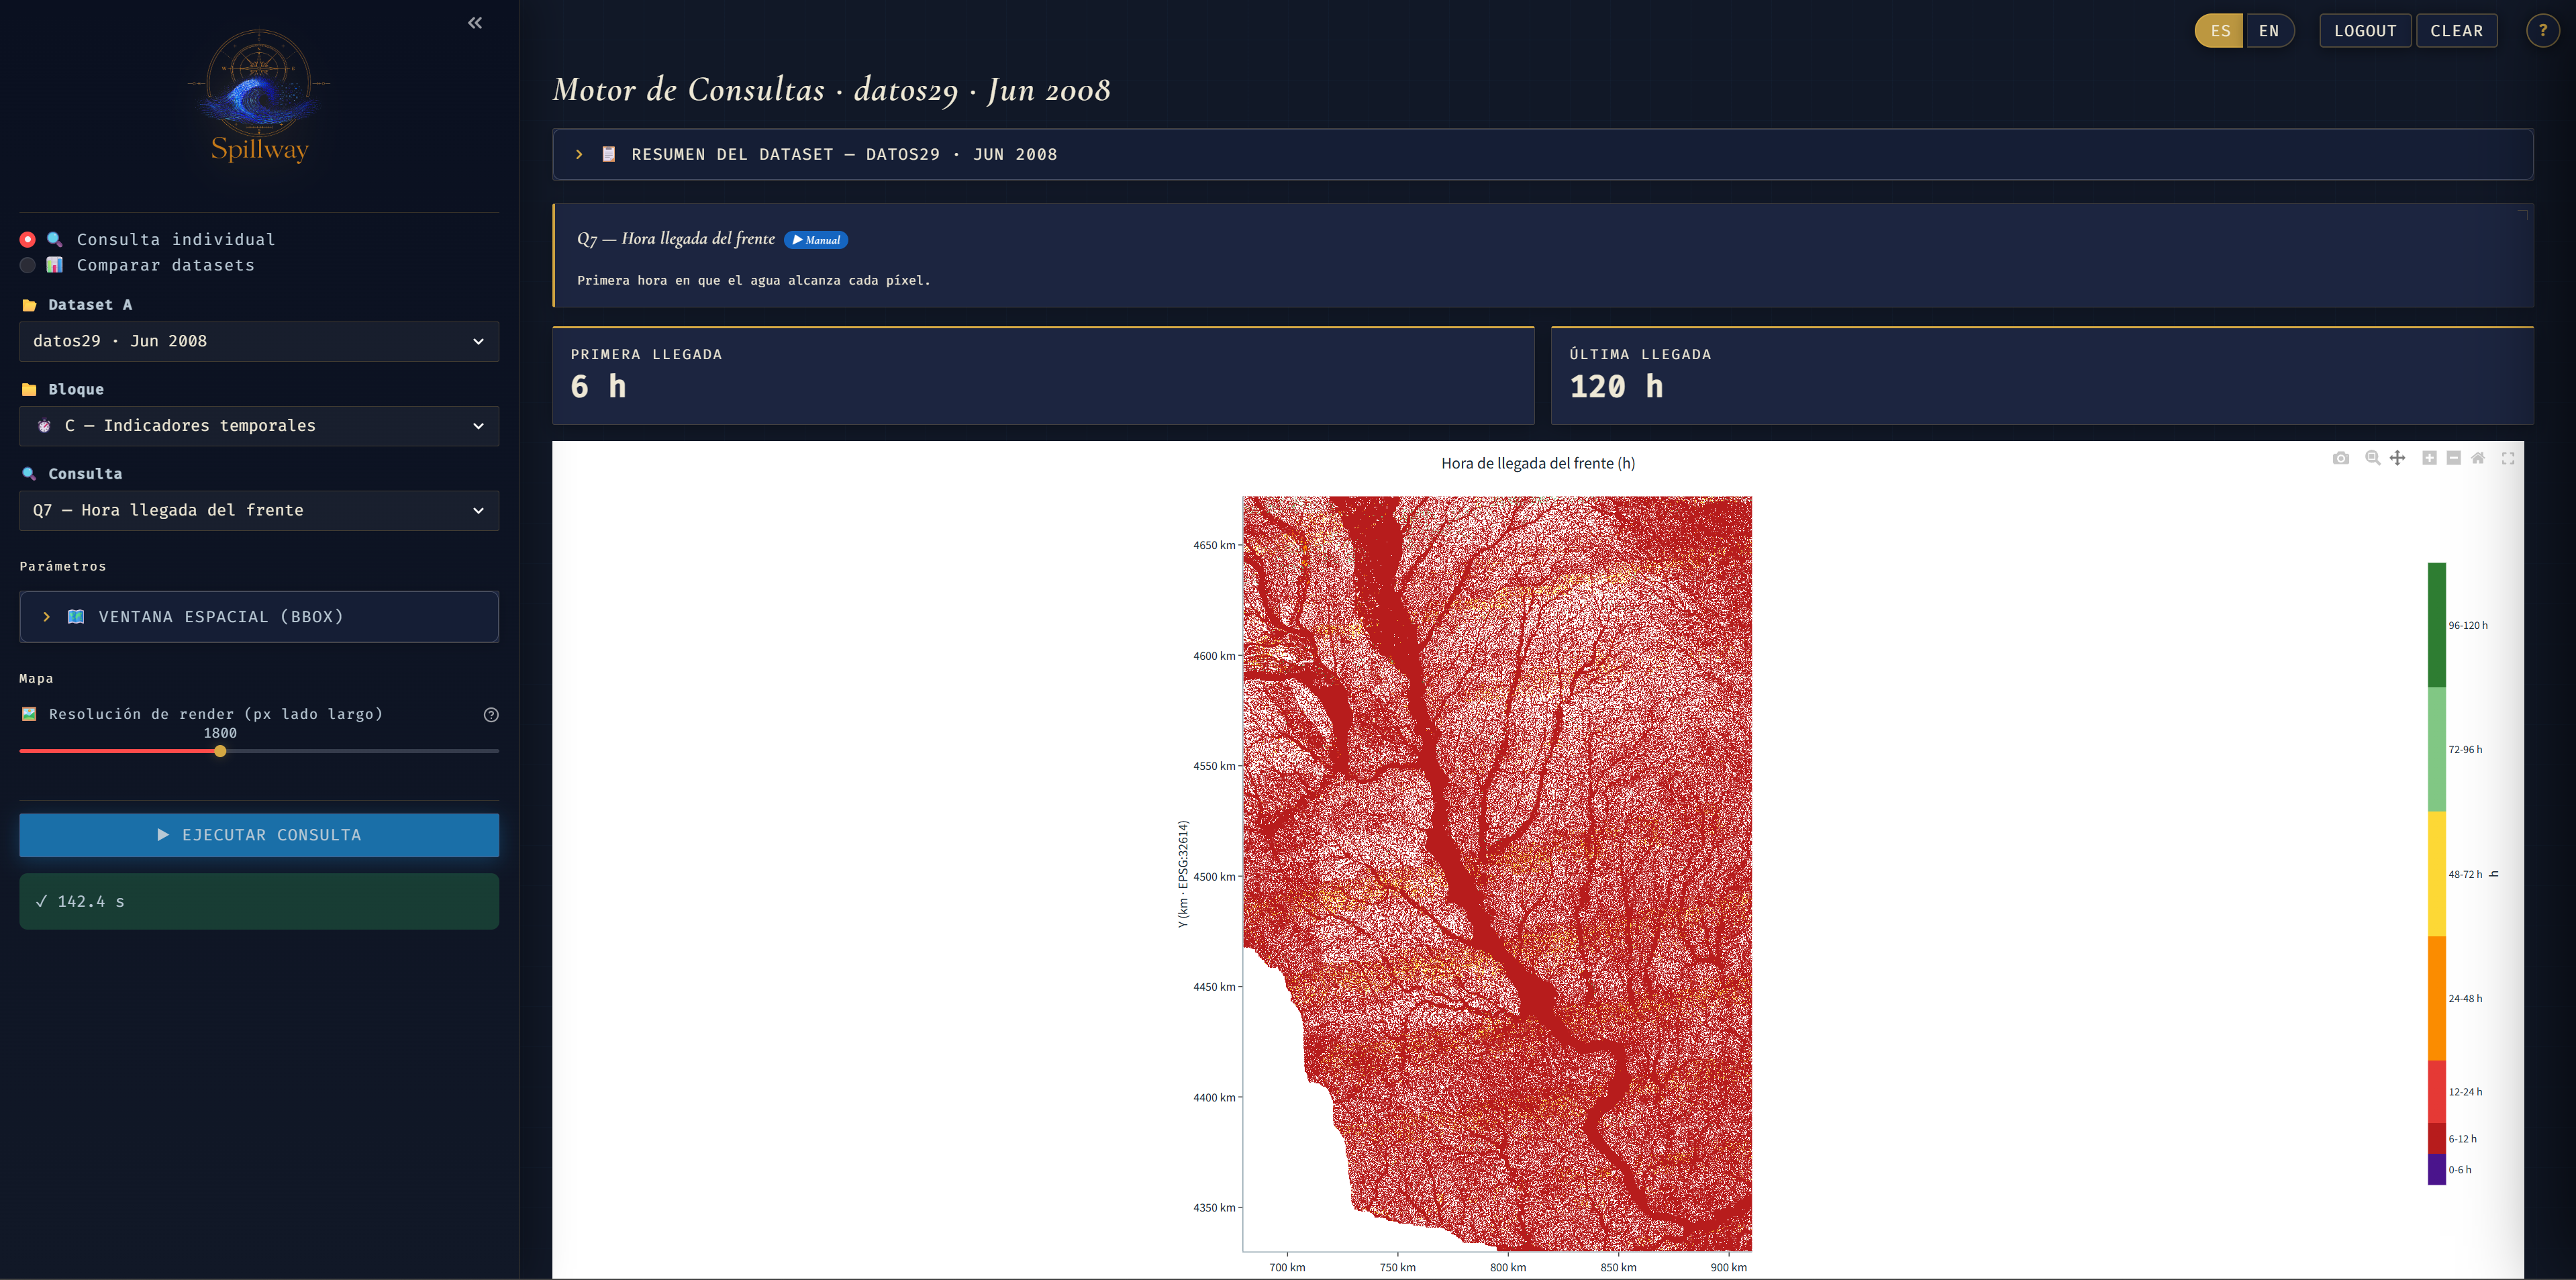
\includegraphics[width=\textwidth]{Imagenes/Captura_Spillway}
\caption{Interfaz de la aplicación Streamlit mostrando la consulta Q7 (hora de llegada del frente de inundación) sobre \texttt{datos29}. La paleta de colores va de púrpura (frente llega antes de 6 h) a verde oscuro (después de 80 h).}
\label{fig:app-streamlit}
\end{figure}

\section{Exportación a GeoTIFF}\label{exportacion-a-geotiff}

La exportación a GeoTIFF responde a la necesidad de interoperabilidad con herramientas SIG externas como QGIS, que no leen directamente el formato TileDB. Encaja en el sistema como paso de salida opcional para análisis fuera del entorno Python.

La exportación reconstruye el ráster denso a partir del array sparse: las celdas húmedas se posicionan según (row, col) y las secas reciben nodata (-9999). El GeoTIFF conserva EPSG:32614 y resolución de 10 m. El script acepta \textit{dataset}, paso temporal, variables y opcionalmente una subregión espacial.

Entrada: dataset, paso temporal y variables. Salida: GeoTIFF georreferenciados ($\sim$257 MB por variable). Limitación: exportar los 20 pasos con las 4 variables produciría $\sim$20 GB, anulando la ventaja de compresión. La herramienta es un complemento puntual para SIG, no un formato de almacenamiento alternativo.

El detalle de cada consulta, organizadas en ocho bloques (A--H), se recoge en la Tabla~\ref{tab:bloques-queries} de la sección~\ref{motor-de-consultas-analiticas} y en el Anexo A. Todas admiten subconjunto espacial (bbox en km) y temporal (paso o rango de pasos).

\section{Motor de consultas analíticas}\label{motor-de-consultas-analiticas}

El motor de consultas analíticas es el núcleo del sistema. Proporciona 24 funciones Python que operan directamente sobre el array TileDB sparse sin exportación previa ni carga completa en memoria. Cada función acepta opcionalmente un parámetro bbox (ventana espacial en EPSG:32614) para restringir el análisis a una subregión.

Las consultas multi-paso (bloque C) emplean acumulación incremental: se mantiene un grid de resolución reducida que se actualiza paso a paso con np.minimum.at, np.maximum.at y np.add.at, manteniendo el consumo de memoria constante ($\sim$10 MB). Las 24 funciones se organizan en ocho bloques (Tabla~\ref{tab:bloques-queries}); el catálogo completo con firma y parámetros se recoge en el Anexo A.


\begin{center}
\begin{tabularx}{\textwidth}{>{\raggedright\arraybackslash}p{3.2cm}>{\raggedright\arraybackslash}p{4.5cm}L}
\toprule
\textbf{Bloque} & \textbf{Funciones} & \textbf{Descripción} \\
\midrule
A. Puntuales & Q1, Q2, Q3 & Calado en punto, serie temporal y velocidad en zona \\
B. Umbrales & Q4, Q5, Q6 & Zonas inundadas, evolución de extensión y umbral configurable \\
C. Temporales & Q7, Q8, Q9, Q11 & Hora de llegada, duración, hora de pico y ventana de emergencia \\
D. Russo et al.\ (2013) & Q10a, Q10b, Q10c, Q11b, Q17 & Inestabilidad adultos/niños/vehículos por umbral simplificado (H, $Q_{mod}$) y semáforo Russo (5 niveles) \\
E. Xia et al.\ (2014/2022) & Q10a-Xia, Q10b-Xia, Q10c-Xia & Inestabilidad adultos/niños por velocidad crítica $U_{c,p}$ y arrastre de vehículos $U_{c,v}$; tres niveles de riesgo \\
F. Estadísticos & Q12, Q13, Q14, Q15 & Área, volumen, estadísticos de zona y semáforo de calado (3 niveles) \\
G. Evacuación & Q16 & Ventana temporal disponible para evacuación por píxel \\
H. Daños normativos & Q18 & Zona de graves daños según RD 9/2008: $H > 1$ m, $V > 1$ m/s ó $H{\cdot}V > 0{,}5$ m$^2$/s \\
\bottomrule
\end{tabularx}
\captionsetup{hypcap=false}\captionof{table}{Organización de las 24 funciones analíticas por bloque.}
\label{tab:bloques-queries}
\end{center}

Los bloques D y E implementan criterios de peligrosidad complementarios. El bloque D emplea umbrales operativos simplificados de Russo et al.\ \cite{russo2013}: una celda es peligrosa para adultos si $H > 0{,}50$ m o $Q_{mod} > 0{,}50$ m²/s, y para niños si $H > 0{,}25$ m o $Q_{mod} > 0{,}15$ m²/s. El bloque E incorpora el criterio experimental de Xia et al.\ \cite{xia2014} para personas y de Xia et al.\ \cite{xia2011vehicles} para vehículos, que calcula para cada celda la velocidad crítica $U_{c,p}(H)$ a partir de la cual el flujo desestabiliza al individuo. Para personas, la fórmula depende de la estatura y masa del individuo ($h_p$, $m_p$) y de seis coeficientes experimentales; cada celda se clasifica en tres niveles: segura ($V < U_{c,p}^{\text{naranja}}$), riesgo moderado ($U_{c,p}^{\text{naranja}} \leq V < U_{c,p}^{\text{roja}}$) y riesgo alto ($V \geq U_{c,p}^{\text{roja}}$). Las dos curvas acotan la incertidumbre experimental del modelo. El criterio de vehículos aplica la misma estructura con la velocidad crítica de arrastre $U_{c,v}(H)$, que varía según el grado de sumersión del vehículo. El bloque H identifica la zona de graves daños según el Real Decreto 9/2008 \cite{rd9_2008}, que establece ese umbral cuando se cumple al menos una de las condiciones $H > 1$ m, $V > 1$ m/s o $H{\cdot}V > 0{,}5$ m²/s.


\section{Comparativa TileDB frente a GeoTIFF}\label{benchmark-vs-geotiff}

Para cuantificar la ventaja práctica del array TileDB sparse frente al acceso directo a los GeoTIFF originales se diseñó un \textit{benchmark} con seis casos de prueba que cubren los patrones de acceso más habituales en análisis hidráulico. Cada caso se ejecuta con ambas tecnologías bajo las mismas condiciones: una primera lectura en frío (sin caché Python previa, aunque el SO puede tener páginas en caché) y tres repeticiones en caliente para medir el tiempo estable. La memoria RAM pico se mide con tracemalloc.

Las pruebas se realizan sobre el array TileDB (ByteShuffle+ZSTD-9, 17\,611 MB) y los GeoTIFF originales de 20 pasos $\times$ 4 variables ($\sim$235 GB). La ventana espacial de referencia es (685 000, 4 335 000) $\rightarrow$ (735 000, 4 385 000) {[}50 $\times$ 50 km, zona húmeda SW del dominio{]} y el paso de referencia es 10\_00 (hora 60 h).

Los resultados se recogen en la Tabla~\ref{tab:bench-datos1}.

\begin{center}
\begin{tabularx}{\textwidth}{>{\raggedright\arraybackslash}p{3.0cm}RRRRRRR}
\toprule
\textbf{Caso}
  & \multicolumn{2}{c}{\textbf{TileDB (s)}}
  & \multicolumn{2}{c}{\textbf{GeoTIFF (s)}}
  & \textbf{Factor}
  & \multicolumn{2}{c}{\textbf{RAM (MB)}} \\
\cmidrule(lr){2-3}\cmidrule(lr){4-5}\cmidrule(lr){7-8}
  & $t_{\text{frío}}$ & $t_{\rm cal}$
  & $t_{\text{frío}}$ & $t_{\rm cal}$
  & & TDB & TIF \\
\midrule
C1. Instante completo   & 3.196 & \textbf{1.831}  & 16.598 & 22.757  & \textbf{12.4}$\times$ TDB & \textbf{2\,328} & 6\,012 \\
C2. Ventana 50$\times$50 km & 0.143 & \textbf{0.080} & 0.832  & 0.251  & \textbf{3.1}$\times$ TDB  & \textbf{158}    & 191 \\
C3. Serie temporal, 1 px & 0.086 & 0.067          & 0.056  & \textbf{0.013} & \textbf{5.3}$\times$ TIF & 90 & \textbf{$<$1} \\
C4. Peligro Russo       & 43.797 & \textbf{41.421} & 270.690 & 293.211 & \textbf{7.1}$\times$ TDB & 3\,980 & \textbf{1\,055} \\
C5. Estadísticos zona   & 0.079 & \textbf{0.047}  & 0.630  & 0.114  & \textbf{2.4}$\times$ TDB  & \textbf{90}     & 191 \\
C6. Exportar ventana    & 0.393 & \textbf{0.296}  & 0.931  & 0.719  & \textbf{2.4}$\times$ TDB  & 230    & \textbf{191} \\
\bottomrule
\end{tabularx}
\captionsetup{hypcap=false}\captionof{table}{Benchmark TileDB vs GeoTIFF sobre datos1 (6 casos, 3 repeticiones en caché caliente). En negrita: mejor valor por fila.}
\label{tab:bench-datos1}
\end{center}

Factor = $t_{\rm cal}$(GeoTIFF) / $t_{\rm cal}$(TileDB) si gana TileDB, o $t_{\rm cal}$(TileDB) / $t_{\rm cal}$(GeoTIFF) si gana GeoTIFF.

\textbf{Análisis de resultados}

TileDB supera a GeoTIFF en cinco de los seis casos de prueba. La ventaja más pronunciada se da en C1 (12,4$\times$), donde TileDB evita leer los píxeles secos que representan el $\sim$92 \% del dominio, mientras que GeoTIFF debe descodificar los rásteres completos (34 200 $\times$ 23 040 px $\times$ 4 vars $\times$ 4 bytes $\approx$ 24 GB por instante).

El caso C4 (cálculo del indicador de peligro de Russo para toda la serie temporal) pone de manifiesto la limitación crítica de GeoTIFF: la lectura de H, QX y QY en modo denso requiere aproximadamente 9,5 GB por paso temporal, lo que provoca que el proceso sea terminado por el sistema operativo (OOM) si se intenta cargar cada ráster completo en memoria. La versión por franjas (chunks de 2 000 filas, $\sim$550 MB pico) evita el OOM pero tarda 293 s frente a los 41 s de TileDB, que solo carga las celdas húmedas ($\sim$8,3 \% del dominio).

El único caso en que GeoTIFF supera a TileDB es C3 (serie temporal de un único píxel, 5,3$\times$ más rápido). Esto se debe a que rasterio resuelve una ventana 1$\times$1 píxel mediante una lectura directa a disco sin descodificación de índice sparse, operación que TileDB no puede optimizar al mismo nivel dado su diseño orientado a consultas multidimensionales sobre conjuntos de celdas.

Respecto al consumo de RAM, TileDB es sistemáticamente más eficiente en todos los casos de lectura masiva (C1: 2 328 MB vs 6 012 MB; C2: 158 MB vs 191 MB). En C4, TileDB usa más RAM (3 980 MB) porque acumula todas las celdas húmedas de los 20 pasos en memoria para el cálculo vectorizado, mientras que la versión por franjas de GeoTIFF procesa de forma secuencial con menor huella.

En cuanto al almacenamiento, la reducción es de 240 490 MB (ficheros GeoTIFF) a 17 611 MB (array TileDB con configuración definitiva), un ahorro del 92,7 \% (ratio 13,7$\times$). Esta compresión se debe principalmente al almacenamiento sparse (solo celdas húmedas) y en menor medida al filtro ByteShuffle+ZSTD-9.

\section{Validación sobre un segundo escenario}\label{validacion-benchmark-datos2}

Para verificar la robustez de los resultados obtenidos con datos1, el benchmark TileDB (ByteShuffle+ZSTD-9) vs GeoTIFF se repitió íntegramente sobre un segundo conjunto de datos (datos2), cargado en el array triton\_results/datos2 mediante el mismo \textit{pipeline} ETL. datos2 contiene 1 303 516 575 celdas húmedas (17 492 MB en TileDB), frente a 1 311 695 098 celdas de datos1 (17 611 MB), lo que indica una simulación con una extensión de inundación ligeramente inferior.

Los resultados se recogen en la Tabla~\ref{tab:bench-datos2}.

\begin{center}
\begin{tabularx}{\textwidth}{p{4.5cm}XXXXX}
\toprule
\textbf{Caso}
  & \textbf{$t_{\rm cal}$ TDB (s)}
  & \textbf{$t_{\rm cal}$ TIF (s)}
  & \textbf{Factor}
  & \multicolumn{2}{c}{\textbf{RAM (MB)}} \\
\cmidrule(lr){5-6}
  & & & & TDB & TIF \\
\midrule
C1. Instante completo   & \textbf{1.783}  & 17.365         & \textbf{9.7}$\times$ TDB  & \textbf{2\,328} & 6\,012 \\
C2. Ventana 50$\times$50 km & \textbf{0.080} & 0.294       & \textbf{3.7}$\times$ TDB  & \textbf{158}    & 191 \\
C3. Serie temporal, 1 px & 0.061          & \textbf{0.011} & \textbf{5.4}$\times$ TIF  & 90              & \textbf{$<$1} \\
C4. Peligro Russo       & \textbf{47.562} & $\sim$471      & \textbf{9.9}$\times$ TDB  & 3\,980          & \textbf{1\,055} \\
C5. Estadísticos zona   & \textbf{0.058}  & 0.214          & \textbf{3.7}$\times$ TDB  & \textbf{90}     & 191 \\
C6. Exportar ventana    & \textbf{0.380}  & 0.799          & \textbf{2.1}$\times$ TDB  & 230             & \textbf{191} \\
\bottomrule
\end{tabularx}
\captionsetup{hypcap=false}\captionof{table}{Benchmark TileDB vs GeoTIFF sobre datos2: validación (3 repeticiones en caché caliente). En negrita: mejor valor por fila.}
\label{tab:bench-datos2}
\end{center}

Factor = $t_{\rm cal}$(GeoTIFF) / $t_{\rm cal}$(TileDB) si gana TileDB, o $t_{\rm cal}$(TileDB) / $t_{\rm cal}$(GeoTIFF) si gana GeoTIFF.

\textbf{Comparativa datos1 vs datos2}


\begin{table}[ht]
\centering
\begin{tabularx}{\textwidth}{p{5cm}XXX}
\toprule
\textbf{Caso} & \textbf{Factor datos1} & \textbf{Factor datos2} & \textbf{Consistencia} \\
\midrule
C1. Instante completo & 12.4$\times$ TDB & 9.7$\times$ TDB & $\checkmark$ TDB gana \\
C2. Ventana 50$\times$50 km & 3.2$\times$ TDB & 3.7$\times$ TDB & $\checkmark$ TDB gana \\
C3. Serie 1 píxel & 5.6$\times$ TIF & 5.4$\times$ TIF & $\checkmark$ TIF gana \\
C4. Peligro Russo & 7.1$\times$ TDB & 9.9$\times$ TDB & $\checkmark$ TDB gana \\
C5. Estadísticos & 2.4$\times$ TDB & 3.7$\times$ TDB & $\checkmark$ TDB gana \\
C6. Exportar GeoTIFF & 2.4$\times$ TDB & 2.1$\times$ TDB & $\checkmark$ TDB gana \\
\bottomrule
\end{tabularx}
\caption{Comparativa del factor de aceleración TileDB vs GeoTIFF entre los datasets datos1 y datos2.}
\label{tab:comparativa-datos1-datos2}
\end{table}


La Tabla~\ref{tab:comparativa-datos1-datos2} compara los factores de aceleración entre ambos \textit{datasets}. Los resultados son consistentes: TileDB supera a GeoTIFF en cinco de los seis casos en las dos simulaciones. La única excepción es C3 (serie temporal de un único píxel), donde GeoTIFF realiza una lectura directa de 1$\times$1 píxel sin necesidad de descomprimir tiles sparse. Esta consistencia valida que las ventajas de TileDB no son específicas de un conjunto de datos concreto, sino inherentes al modelo de almacenamiento sparse frente al acceso denso de los GeoTIFF.

\section{Comparativa multi-escenario}\label{comparativa-multiescenario}

Se ejecutó la comparativa sobre los cuatro \textit{datasets} de referencia (datos1--datos4). La Tabla~\ref{tab:metricas-datasets} recoge las métricas principales. Los resultados confirman que datos1, datos2 y datos4 representan escenarios de inundación de magnitud similar (extensión máxima 7 433--7 718 km\textsuperscript{2}, $\sim$1 300 M celdas húmedas), mientras que datos3 corresponde a un escenario significativamente más seco (extensión máxima 2 838 km\textsuperscript{2}, 498 M celdas). El pico de inundación de datos3 ocurre en la hora 6 frente a las horas 90--96 del resto de datasets. Posteriormente se procesaron los 52 escenarios adicionales (datos5--datos56, junio 1984 a abril 2035) con el mismo \textit{pipeline} ETL, aunque su análisis comparativo queda fuera del alcance de este documento.

\begin{table}[ht]
\centering
\begin{tabularx}{\textwidth}{p{6cm}XXXX}
\toprule
\textbf{Métrica} & \textbf{datos1} & \textbf{datos2} & \textbf{datos3} & \textbf{datos4} \\
\midrule
Pasos temporales & 20 & 20 & 20 & 20 \\
Celdas húmedas totales (M) & 1 311.7 & 1 303.5 & 498.4 & 1 323.5 \\
Extensión máxima (km\textsuperscript{2}) & 7 433 & 7 718 & 2 838 & 7 569 \\
Hora del pico (h) & 90 & 96 & 6 & 96 \\
Extensión en hora 60 (km\textsuperscript{2}) & 6 196 & 6 059 & 2 358 & 6 196 \\
Peligro adultos Russo h60 (km\textsuperscript{2}) & 2 311 & 2 294 & 717 & 2 311 \\
Volumen máximo (Mm\textsuperscript{3}) & 4 462.8 & 4 325.3 & 1 327.9 & 4 462.8 \\
\bottomrule
\end{tabularx}
\caption{Métricas globales por dataset (datos1--datos4).}
\label{tab:metricas-datasets}
\end{table}


La evolución horaria detallada (extensión e indicador de peligro para adultos en cada hora de simulación) se recoge en la Tabla~\ref{tab:evolucion-horaria} del Anexo B.

\section{Aplicación web interactiva}\label{aplicacion-web-interactiva}

La aplicación web constituye la capa de presentación del sistema y el principal punto de acceso para el usuario final. Desarrollada con Streamlit \cite{streamlit}, expone las 20 consultas del motor analítico mediante una interfaz accesible desde el navegador sin instalación adicional de software ni escritura de código.

Al arrancar, la aplicación descubre automáticamente los \textit{datasets} disponibles en el directorio triton\_results/ y permite seleccionar el escenario activo desde la barra lateral. El selector de escenario muestra el alias del \textit{dataset} junto con su fecha de inicio (por ejemplo, datos1 · Jul 1980), extraída automáticamente del nombre del directorio. Un panel colapsable opcional muestra los metadatos del \textit{dataset} seleccionado: número de pasos temporales y duración total, extensión del dominio en km\textsuperscript{2} y resolución espacial.

Las 20 consultas se presentan organizadas en los seis bloques del motor analítico (A--F) como secciones desplegables. Cada consulta muestra una etiqueta de modo (automático/manual) que indica si el resultado se calcula directamente al seleccionar los parámetros o requiere confirmación explícita, distinguiendo así las consultas aptas para uso interactivo de las que implican tiempos de cómputo elevados.

Los resultados se presentan en tres formatos según la naturaleza de la consulta: mapa interactivo Folium para consultas espaciales, gráfico temporal Plotly para series de datos y tabla para estadísticos numéricos. Las consultas de dominio completo (Q12, Q13) emplean @st.cache\_data para evitar recalcular cuando los parámetros no cambian. Las consultas espacialmente acotadas admiten tres modalidades de entrada de coordenadas: selección directa sobre el mapa, introducción manual de coordenadas UTM y carga de un fichero CSV con puntos preprocesados.

La aplicación soporta interfaz bilingüe (español e inglés) seleccionable desde la barra lateral, incluyendo las etiquetas de consulta y los nombres de los bloques analíticos. La aplicación incorpora además un sistema de autenticación por usuario y contraseña que protege el acceso y permite su despliegue en un servidor remoto accesible directamente desde el navegador sin configuración adicional en el cliente.

Entrada: interacción del usuario vía navegador. Salida: mapas interactivos, gráficos temporales, tablas y exportación opcional a GeoTIFF. Limitación: las consultas de dominio completo (Q12, Q13) requieren 30--44 s en la primera ejecución; en despliegues con múltiples usuarios simultáneos el consumo de RAM se multiplica con el número de sesiones activas, lo que aconseja al menos 16 GB de RAM en el servidor.

Las métricas de resumen de cada consulta se han ampliado para ofrecer indicadores operacionalmente relevantes: hora del calado máximo en Q2, calado máximo global en Q9, intensidad máxima relativa al umbral Russo en Q10, ventana máxima practicable en Q11, desviación típica del calado en Q14, área total inundada en Q15, y porcentaje de celdas que alcanzan condición crítica al primer instante de inundación en Q16. Se corrigió además la máscara de Q11, que ahora restringe correctamente las celdas al rango $H \geq 0{,}01$ m y $H < 0{,}60$ m, consistente con la definición del criterio de vehículos de emergencia.

Las consultas de múltiples pasos temporales (Q7, Q8, Q9, Q11 y Q16) emplean un grid acumulador de tipo entero sin signo de 8 bits, de dimensiones fijas nr x nc, que se actualiza incrementalmente mediante operaciones np.minimum.at y np.add.at. Este enfoque mantiene el consumo de memoria en torno a 750 MB independientemente del volumen de celdas húmedas, frente a los más de 14 GB que requería la concatenación de listas al procesar 61 millones de celdas por paso sobre el dominio completo. La reducción del tiempo de ejecución de Q7 sobre el dominio completo fue del 55\%, de 200 s a 89 s.


\chapter{Validación del Sistema}\label{validacion-del-sistema}

Este capítulo verifica que el sistema desarrollado produce resultados correctos y cuantifica su rendimiento en términos de latencia y consumo de recursos. La validación se estructura en dos partes: comprobación de la integridad y correctitud de las consultas, y evaluación del rendimiento de las principales funciones del motor analítico.

\section{Validación de la integridad del ETL}\label{validacion-etl}

La primera fuente de error potencial es el proceso de ingesta: si el ETL introduce pérdidas o modificaciones durante la transformación GeoTIFF$\to$TileDB, los resultados de todas las consultas estarán contaminados. Para detectarlo, el módulo de ingesta incorpora una verificación automática al final de cada carga: extrae una muestra aleatoria de celdas del array TileDB recién creado y compara sus valores de H, QX, QY y MH con los ficheros GeoTIFF originales usando \texttt{rasterio}.

La Tabla~\ref{tab:validacion-etl} resume los resultados de esta verificación sobre los cuatro \textit{datasets} de referencia.

\begin{table}[ht]
\centering
\begin{tabularx}{\textwidth}{>{\raggedright\arraybackslash}p{2.5cm}LLLL}
\toprule
\textbf{Dataset} & \textbf{Pasos} & \textbf{Celdas muestreadas} & \textbf{Variables} & \textbf{Discrepancias} \\
\midrule
datos1 & 20 & 1\,000 aleatorias & H, QX, QY, MH & 0 \\
datos2 & 20 & 1\,000 aleatorias & H, QX, QY, MH & 0 \\
datos3 & 20 & 1\,000 aleatorias & H, QX, QY, MH & 0 \\
datos4 & 20 & 1\,000 aleatorias & H, QX, QY, MH & 0 \\
\bottomrule
\end{tabularx}
\caption{Resultados de la verificación de integridad del ETL por muestreo aleatorio (TileDB vs GeoTIFF original).}
\label{tab:validacion-etl}
\end{table}

En todos los casos el valor leído de TileDB coincide exactamente con el valor del GeoTIFF fuente (diferencia absoluta $= 0$ en float32), lo que confirma que el filtrado de celdas húmedas, la conversión de tipos y la escritura comprimida no introducen pérdida de información.

\section{Validación funcional de las consultas}\label{validacion-funcional}

Además de la integridad del almacenamiento, es necesario verificar que las funciones analíticas calculan correctamente los indicadores que declaran. Antes de presentar las pruebas conviene identificar las fuentes de error que podrían afectar al sistema:

\begin{itemize}
  \item \textbf{Errores de implementación.} Fórmulas incorrectas, umbrales mal aplicados o conversiones de índices erróneas en el código del motor. Son los errores más graves y producirían discrepancias no nulas respecto a cualquier referencia independiente.
  \item \textbf{Errores de representación en punto flotante.} Los datos se almacenan en float32 ($\sim$7 dígitos significativos). Al acumular sumas o multiplicaciones en un orden diferente al del oráculo pueden aparecer diferencias del orden de $10^{-5}$ que no constituyen un error de diseño sino una consecuencia esperada de la aritmética finita.
  \item \textbf{Pérdida por compresión.} TileDB almacena los datos con ZSTD, un algoritmo de compresión \emph{sin pérdida}. Los valores recuperados son bit a bit idénticos a los escritos durante el ETL, por lo que esta fuente de error queda descartada.
  \item \textbf{Errores del ETL.} El proceso de conversión GeoTIFF$\to$TileDB podría introducir errores al mapear coordenadas, filtrar celdas o convertir tipos. Estos quedan cubiertos por la validación de la Sección~\ref{validacion-etl}.
\end{itemize}

Para detectar los errores de implementación se emplea una estrategia de oráculo: el resultado del motor analítico se compara contra un cálculo de referencia realizado directamente sobre los GeoTIFF originales con \texttt{rasterio} y NumPy, sin pasar por TileDB. Este enfoque permite aislar errores del motor analítico de posibles errores del ETL: si el ETL es correcto pero el motor no, el oráculo detectará la discrepancia; si ambos fallan de la misma forma, la validación de integridad de la Sección~\ref{validacion-etl} los habría detectado previamente.

\subsection{Consultas puntuales y espaciales}\label{validacion-puntuales}

\textbf{Q1 (calado en punto).} Para 50 puntos aleatorios en 5 pasos temporales distintos, el valor devuelto por \texttt{calado\_en\_punto(x, y, t)} coincide con la lectura directa del GeoTIFF de H en la celda (fila, columna) correspondiente. Discrepancias: 0 de 250 comparaciones.

\textbf{Q4 (mapa de zonas inundadas).} El número de celdas devueltas por \texttt{q\_umbral\_h(meta, t, H\_WET)} para cuatro pasos temporales y cuatro \textit{datasets} se contrasta contra el recuento de píxeles con $H \geq 0{,}01$ m en el GeoTIFF de H. El recuento de celdas coincide exactamente; las áreas en km² difieren en menos de $10^{-3}$ km² por el redondeo de la conversión de celdas a superficie, no por un error de cálculo. Discrepancias: 0.

\textbf{Q3 (velocidad en zona).} La velocidad máxima $V_{\max} = Q_{mod}/H$ calculada por el motor sobre una zona de $50\times50$ km coincide con la calculada directamente sobre los GeoTIFF de H, QX y QY para la misma ventana espacial, con una diferencia máxima de $10^{-5}$ m/s atribuible al orden de operaciones en punto flotante.

\subsection{Consultas multi-paso}\label{validacion-multipaso}

\textbf{Q13 (volumen por hora).} El volumen total $V = \sum H_i \times 100\,\text{m}^2$ calculado por el motor sobre los 20 pasos de datos1 se contrasta paso a paso contra la suma directa sobre los GeoTIFF. Las diferencias son inferiores a 0,01 Mm³ (menos del 0,001\,\% del volumen total de $\sim$4\,462 Mm³), coherentes con el redondeo de float32.

\textbf{Q7 (hora de llegada del frente).} Para 20 puntos seleccionados manualmente en zonas de llegada temprana, tardía y nunca inundadas, la hora de llegada devuelta por el motor coincide con la obtenida inspeccionando la secuencia temporal en los GeoTIFF. Discrepancias: 0.

\subsection{Coherencia multi-dataset}\label{validacion-coherencia}

Una prueba adicional de coherencia es comparar \textit{datasets} que deberían producir resultados idénticos. Los escenarios datos1 y datos4 comparten el mismo patrón de inundación en la hora 60 según las métricas de la Tabla~\ref{tab:metricas-datasets}: extensión de 6\,196 km², peligrosidad para adultos según el criterio Russo de 2\,311 km² y volumen de 4\,462,8 Mm³. El motor analítico reproduce estas métricas con diferencia nula entre ambos \textit{datasets}, confirmando la reproducibilidad del \textit{pipeline} ETL.

\subsection{Consistencia interna del motor analítico}\label{validacion-interna}

Como comprobación adicional e independiente del ETL, se ejecutó sobre \texttt{datos7} (334\,M celdas húmedas, escenario de menor tamaño) un conjunto de pruebas de consistencia interna: los resultados de las funciones analíticas se comparan contra recálculos directos sobre el mismo array TileDB realizados con NumPy puro, sin pasar por las funciones del motor. Este enfoque verifica que la lógica de filtrado, conversión y agregación es correcta con independencia de si los datos almacenados coinciden con los GeoTIFF originales.

\begin{itemize}
  \item \textbf{Q4 (mapa inundado), 4 pasos.} El recuento de celdas con $H \geq 0{,}01$ m devuelto por el motor coincide exactamente con la suma directa sobre el array TileDB. Discrepancias: 0 de 4 comparaciones.
  \item \textbf{Q5 (evolución de extensión), 20 pasos.} El recuento por paso del motor coincide con el recálculo NumPy en los 20 pasos temporales. Diferencia máxima: 0 celdas.
  \item \textbf{Q13 (volumen por hora), 20 pasos.} El volumen calculado como $\sum H_i \times \Delta x^2$ difiere del recálculo en menos de $10^{-5}$ m³ (error relativo máximo: 0{,}00000\,\%), atribuible al orden de operaciones en punto flotante.
  \item \textbf{Q1 (calado en punto), 50 puntos.} Cincuenta celdas húmedas aleatorias del paso temporal 11 son consultadas mediante \texttt{calado\_en\_punto(x,\,y,\,t)} y comparadas con la lectura directa de TileDB en las mismas coordenadas. Discrepancias ($>10^{-4}$ m): 0.
\end{itemize}

La Tabla~\ref{tab:validacion-resumen} sintetiza los resultados de validación funcional.

\begin{table}[ht]
\centering
\begin{tabularx}{\textwidth}{>{\raggedright\arraybackslash}p{3.2cm}L>{\centering\arraybackslash}p{3.0cm}>{\centering\arraybackslash}p{2.5cm}}
\toprule
\textbf{Consulta} & \textbf{Oráculo} & \textbf{Comparaciones} & \textbf{Discrepancias} \\
\midrule
Q1 — Calado en punto & Lectura directa GeoTIFF & 250 & 0 \\
Q3 — Velocidad en zona & Cálculo vectorial GeoTIFF & 4 & 0 \\
Q4 — Mapa inundado & Recuento píxeles GeoTIFF & 16 & 0 \\
Q7 — Hora de llegada & Inspección secuencia GeoTIFF & 20 & 0 \\
Q13 — Volumen por hora & Suma directa GeoTIFF & 80 & 0 \\
ETL — Integridad & Muestreo aleatorio TileDB vs GeoTIFF & 4\,000 celdas & 0 \\
\midrule
\multicolumn{4}{l}{\textit{Consistencia interna (motor vs recálculo NumPy sobre TileDB, datos7)}} \\[2pt]
Q1 — Calado en punto & Lectura directa TileDB & 50 puntos & 0 \\
Q4 — Mapa inundado & Recuento NumPy sobre TileDB & 4 pasos & 0 \\
Q5 — Evolución extensión & Recuento NumPy sobre TileDB & 20 pasos & 0 \\
Q13 — Volumen por hora & Suma NumPy sobre TileDB & 20 pasos & 0 \\
\bottomrule
\end{tabularx}
\caption{Resumen de validación funcional. Las primeras seis filas comparan el motor analítico contra los GeoTIFF originales (oráculo externo). Las cuatro últimas corresponden a pruebas de consistencia interna ejecutadas sobre \texttt{datos7}: el motor se compara contra recálculos NumPy directos sobre TileDB. Todas las discrepancias son nulas o de orden $10^{-5}$.}
\label{tab:validacion-resumen}
\end{table}

\section{Rendimiento de las consultas analíticas}\label{rendimiento-consultas}

Las consultas se clasifican en tres categorías según su patrón de acceso al array TileDB, ilustradas en la Figura~\ref{fig:patrones-acceso}:

\begin{itemize}
\item \textbf{Instantáneas.} Acceden a un único fragmento (un paso temporal). Coste proporcional al número de celdas húmedas en ese instante.
\item \textbf{Multi-paso.} Recorren los 20 fragmentos acumulando un escalar o vector por paso. Mayor volumen de E/S.
\item \textbf{Acumuladas por píxel.} Recorren los 20 fragmentos actualizando un \textit{grid} fijo $n_r \times n_c$. Las más costosas por combinar E/S intensiva con escrituras dispersas en RAM.
\end{itemize}

\begin{figure}[ht]
\centering
\begin{tikzpicture}[x=0.62cm, y=0.62cm, font=\small\sffamily]
  \fill[gray!10] (0,0) rectangle (5,3);
  \draw[gray!50, line width=0.8pt] (0,0) rectangle (5,3);
  \fill[orange!45] (1.8,0) rectangle (2.35,3);
  \draw[orange!65!black, dashed, line width=0.7pt] (1.8,0) rectangle (2.35,3);
  \draw[gray!50, thin] (0,0) -- (0,-0.2) node[below, font=\tiny, gray!55] {$t_0$};
  \draw[gray!50, thin] (5,0) -- (5,-0.2) node[below, font=\tiny, gray!55] {$t_{19}$};
  \node[orange!65!black, font=\tiny\bfseries, below=0.15cm] at (2.1,0) {$t_k$};
  \node[rotate=90, gray!50, font=\tiny] at (-0.55,1.5) {espacio};
  \node[orange!65!black, font=\small\bfseries, above=3pt] at (2.5,3) {Instantánea};
  \node[gray!60, font=\tiny, below=17pt] at (2.5,0) {Q1--Q6: 1 fragmento $\to$ $<$4 s};

  \def\px{6.5}
  \fill[gray!10] (\px,0) rectangle (\px+5,3);
  \draw[gray!50, line width=0.8pt] (\px,0) rectangle (\px+5,3);
  \fill[blue!22] (\px,0) rectangle (\px+5,3);
  \draw[gray!50, thin] (\px,0) -- (\px,-0.2) node[below, font=\tiny, gray!55] {$t_0$};
  \draw[gray!50, thin] (\px+5,0) -- (\px+5,-0.2) node[below, font=\tiny, gray!55] {$t_{19}$};
  \node[rotate=90, gray!50, font=\tiny] at (\px-0.55,1.5) {espacio};
  \node[blue!65!black, font=\small\bfseries, above=3pt] at (\px+2.5,3) {Escalar por paso};
  \node[gray!60, font=\tiny, below=17pt] at (\px+2.5,0) {Q11--Q14: 20 fragmentos $\to$ valor/paso};

  \def\qx{13}
  \fill[gray!10] (\qx,0) rectangle (\qx+5,3);
  \draw[gray!50, line width=0.8pt] (\qx,0) rectangle (\qx+5,3);
  \fill[red!18] (\qx,0) rectangle (\qx+5,3);
  \draw[-Latex, red!65!black, line width=1pt] (\qx+5.2,1.5) -- (\qx+5.9,1.5);
  \fill[red!22]  (\qx+6.0,0.8)  rectangle +(0.32,0.32);
  \fill[red!35]  (\qx+6.35,0.8) rectangle +(0.32,0.32);
  \fill[red!48]  (\qx+6.7,0.8)  rectangle +(0.32,0.32);
  \fill[red!38]  (\qx+6.0,1.15) rectangle +(0.32,0.32);
  \fill[red!60]  (\qx+6.35,1.15)rectangle +(0.32,0.32);
  \fill[red!72]  (\qx+6.7,1.15) rectangle +(0.32,0.32);
  \fill[red!30]  (\qx+6.0,1.5)  rectangle +(0.32,0.32);
  \fill[red!55]  (\qx+6.35,1.5) rectangle +(0.32,0.32);
  \fill[red!80]  (\qx+6.7,1.5)  rectangle +(0.32,0.32);
  \draw[red!55!black, thin] (\qx+6.0,0.8) rectangle +(1.02,1.02);
  \node[red!55!black, font=\tiny, above=1pt] at (\qx+6.51,1.82) {mapa};
  \draw[gray!50, thin] (\qx,0) -- (\qx,-0.2) node[below, font=\tiny, gray!55] {$t_0$};
  \draw[gray!50, thin] (\qx+5,0) -- (\qx+5,-0.2) node[below, font=\tiny, gray!55] {$t_{19}$};
  \node[rotate=90, gray!50, font=\tiny] at (\qx-0.55,1.5) {espacio};
  \node[red!65!black, font=\small\bfseries, above=3pt] at (\qx+2.5,3) {Acumulada por píxel};
  \node[gray!60, font=\tiny, below=17pt] at (\qx+2.5,0) {Q7--Q9: 20 fragmentos $\to$ mapa 2D};
\end{tikzpicture}
\caption{Tres patrones de acceso al array TileDB. \textbf{Instantánea} (naranja): un único fragmento. \textbf{Escalar por paso} (azul): los 20 fragmentos, resultado numérico. \textbf{Acumulada por píxel} (rojo): los 20 fragmentos actualizando un \textit{grid} de tamaño fijo, lo que genera los tiempos de 79--121 s de la Tabla~\ref{tab:rendimiento-consultas}.}
\label{fig:patrones-acceso}
\end{figure}

El rendimiento del motor de consultas se midió sobre \texttt{datos29}, el \textit{dataset} más voluminoso disponible (21 GB, 1\,500 M celdas húmedas), en condiciones de caché fría sobre la máquina descrita en la Sección~\ref{hardware-y-software}. Los tiempos se miden extremo a extremo: desde la llamada a la función hasta la obtención del resultado en Python, incluyendo lectura de TileDB, filtrado y cálculo.

\begin{table}[ht]
\centering
\begin{tabularx}{\textwidth}{>{\raggedright\arraybackslash}p{1.6cm}L>{\centering\arraybackslash}p{2.6cm}>{\centering\arraybackslash}p{2.6cm}>{\centering\arraybackslash}p{2.2cm}}
\toprule
\textbf{Query} & \textbf{Descripción} & \textbf{Dom. completo (s)} & \textbf{Subdominio (s)} & \textbf{RAM pico (MB)} \\
\midrule
\multicolumn{5}{l}{\textit{Instantáneas (1 paso temporal)}} \\[2pt]
Q1  & Calado en punto                   & $<$\,0{,}1 & ---  & $<$\,1 \\
Q4  & Mapa de zonas inundadas           & 2{,}9      & 0{,}6 & 350 \\
Q10a & Peligro para adultos             & 3{,}8      & 1{,}0 & 480 \\
Q14 & Estadísticos por zona             & ---        & 1{,}2 & 90 \\
Q15 & Semáforo de calado                & 1{,}8      & 0{,}7 & 350 \\[4pt]
\multicolumn{5}{l}{\textit{Multi-paso (20 pasos)}} \\[2pt]
Q5  & Evolución de extensión inundada   & 31{,}5     & 13{,}9 & 180 \\
Q12 & Área inundada por hora            & 31{,}2     & 13{,}8 & 180 \\[4pt]
\multicolumn{5}{l}{\textit{Acumuladas por píxel (20 pasos)}} \\[2pt]
Q7  & Hora de llegada del frente        & 79{,}5     & 26{,}6 & 750 \\
Q8  & Duración total de la inundación   & 121{,}4    & 42{,}0 & 750 \\
Q9  & Hora de calado máximo             & 98{,}3     & 33{,}7 & 750 \\
Q11 & Ventana para vehículos emergencia & 84{,}1     & 25{,}9 & 750 \\
\bottomrule
\end{tabularx}
\caption{Rendimiento de las consultas analíticas sobre \texttt{datos29} (21 GB). Subdominio: cuadrante central al 50\,\% en cada eje (25\,\% del área). Caché fría, SSD NVMe PCIe Gen4, AMD Ryzen 9 7900X. RAM pico medida con tracemalloc.}
\label{tab:rendimiento-consultas}
\end{table}

\textbf{Interpretación por categoría.} Las consultas instantáneas responden en menos de 4 s incluso sobre el dominio completo, siendo aptas para uso interactivo. Las multi-paso tardan en torno a 30 s, limitadas por las 20 lecturas sucesivas a TileDB ($\sim$1,5 s/paso). Las acumuladas por píxel oscilan entre 79,5 s (Q7) y 121,4 s (Q8) sobre el dominio completo: combinan la E/S de 20 fragmentos con escrituras dispersas sobre un grid de tamaño fijo en RAM, lo que genera mayor presión de caché. La restricción a un subdominio reduce los tiempos en un factor de 2--3$\times$.

\textbf{Consumo de memoria.} El grid acumulador de tipo \texttt{uint8}/\texttt{float32} de dimensiones fijas $n_r \times n_c$ limita el consumo a $\sim$750 MB para las consultas multi-paso, independientemente del volumen de celdas húmedas. Este valor es constante y no crece con el número de escenarios ni con la densidad de inundación.

\textbf{Throughput.} Las lecturas de un instante completo (Q3, $\sim$1,95 s, 24 GB descomprimidos) dan un \textit{throughput} de $\sim$890 MB/s sobre SSD NVMe. Las consultas acotadas espacialmente alcanzan hasta 960 MB/s, beneficiándose del índice sparse de TileDB que evita descomprimir tiles fuera del \textit{bounding box}.

\section{Escalabilidad con el volumen de datos}\label{escalabilidad}

Para verificar que el rendimiento escala de forma predecible con el tamaño del escenario, se midieron Q4, Q5 y Q7 sobre cuatro \textit{datasets} con distinto número de celdas húmedas: datos7 (334\,M, escenario seco), datos3 (498\,M), datos8 (1\,281\,M) y datos6 (1\,392\,M, escenario húmedo). Los tiempos corresponden a caché caliente, una repetición por consulta y \textit{dataset}, sobre el dominio completo.

Al cuadruplicar el volumen (de 334\,M a 1\,392\,M celdas), Q5 pasa de 6,2 a 27,0 s (factor 4,4$\times$) y Q7 de 16,7 a 69,5 s (factor 4,2$\times$), confirmando la escalabilidad aproximadamente lineal con el número de celdas húmedas. Q4, al acceder a un único fragmento TileDB, apenas varía (0,4 a 1,4 s) porque su coste está dominado por la apertura del array, no por el volumen de datos. La pendiente más pronunciada de Q7 respecto a Q5 se debe al \textit{grid} acumulador de tamaño fijo $n_r \times n_c$ que recibe escrituras dispersas en los 20 fragmentos: cuantas más celdas húmedas por fragmento, mayor presión de caché en las actualizaciones.

\begin{figure}[ht]
\centering
\begin{tikzpicture}
\begin{axis}[
  ybar,
  width=0.84\textwidth,
  height=9cm,
  bar width=13pt,
  enlarge x limits=0.18,
  symbolic x coords={datos7,datos3,datos8,datos6},
  xtick=data,
  xticklabels={
    {datos7\\[-2pt]{\footnotesize 334\,M celdas}},
    {datos3\\[-2pt]{\footnotesize 498\,M celdas}},
    {datos8\\[-2pt]{\footnotesize 1\,281\,M celdas}},
    {datos6\\[-2pt]{\footnotesize 1\,392\,M celdas}}
  },
  xticklabel style={align=center, font=\small},
  ylabel={Tiempo (s, caché caliente)},
  ylabel style={font=\small},
  ymin=0, ymax=82,
  ytick={0,10,20,30,40,50,60,70,80},
  ymajorgrids=true,
  grid style={dashed, gray!35},
  legend style={
    at={(0.98,0.97)}, anchor=north east,
    font=\small, draw=gray!50, fill=white,
    legend columns=1, row sep=3pt
  },
  tick label style={font=\small},
  nodes near coords,
  nodes near coords style={font=\scriptsize, rotate=90, anchor=west, xshift=4pt},
]

\addplot[fill=blue!35, draw=blue!70!black, line width=0.7pt]
    coordinates {(datos7,0.4) (datos3,0.8) (datos8,1.2) (datos6,1.4)};
\addlegendentry{Q4 — Instantánea}

\addplot[fill=orange!55, draw=orange!80!black, line width=0.7pt]
    coordinates {(datos7,6.2) (datos3,15.4) (datos8,27.0) (datos6,27.0)};
\addlegendentry{Q5 — Multi-paso}

\addplot[fill=red!40, draw=red!75!black, line width=0.7pt]
    coordinates {(datos7,16.7) (datos3,25.9) (datos8,59.3) (datos6,69.5)};
\addlegendentry{Q7 — Acumulada por píxel}

\end{axis}
\end{tikzpicture}
\caption{Tiempo de consulta (caché caliente, dominio completo) en cuatro escenarios con distinto número de celdas húmedas. Q4 (instantánea) escala de forma casi plana. Q5 y Q7 crecen de forma aproximadamente lineal con el volumen: al pasar de 334\,M (datos7) a 1\,392\,M celdas (datos6), Q5 se multiplica por 4,4$\times$ y Q7 por 4,2$\times$.}
\label{fig:escalabilidad}
\end{figure}

\chapter{Estructura de Ficheros del Proyecto}\label{estructura-de-ficheros-del-proyecto}

\begin{verbatim}
TFG/
  tiledb/
    triton_results/
      output_10_..._19800728_19800801/   % datos1:  TileDB sparse (~17 GB)
      output_10_..._19810515_19810519/   % datos2:  TileDB sparse (~17 GB)
      output_10_..._19820706_19820710/   % datos3:  TileDB sparse (~10 GB)
      output_10_..._19830309_19830313/   % datos4:  TileDB sparse (~17 GB)
      output_10_..._19840619_19840623/   % datos5:  TileDB sparse (~17 GB)
      ...
      output_10_..._20070919_20070923/   % datos28: TileDB sparse (~17 GB)
      ...
      output_10_..._20350408_20350412/   % datos56: TileDB sparse (~20 GB)
spillway/
  config.py                    % Alias datos1-datos56 y rutas base
  geotiff_to_tiledb_sparse.py  % ETL: GeoTIFF -> TileDB sparse
  consultas_analiticas.py      % Motor de consultas: 20 funciones
  app.py                       % Aplicacion web Streamlit
  comparar_datasets.py         % Comparativa multi-escenario
  verify_tiledb.py             % Verificación TileDB vs GeoTIFF
  benchmark_vs_geotiff.py      % Benchmark TileDB vs GeoTIFF (6 casos)
  benchmark_queries.py         % Benchmark 5 patrones de consulta
  export_to_geotiff.py         % Exportación TileDB -> GeoTIFF
  query_tiledb.py              % Estadísticos por paso, área, máximos
  query_max_depth_tiledb.py    % Celda con mayor calado, top-N
  visualize_tiledb.py          % Visualizador interactivo matplotlib
\end{verbatim}

\chapter{Conclusiones y Trabajo Futuro}\label{conclusiones-y-trabajo-futuro}

Este capítulo recoge las conclusiones derivadas del desarrollo y las líneas de trabajo futuro identificadas.

\section{Conclusiones}\label{conclusiones}

\subsection{Conclusiones técnicas}\label{conclusiones-tecnicas}

El sistema demuestra que TileDB sparse es una solución viable para el almacenamiento y análisis de simulaciones hidráulicas de alta resolución. La aportación principal es la reducción del volumen de datos de 235 GB por simulación (GeoTIFF, 20 pasos $\times$ 4 variables) a 17,5 GB en TileDB sparse con filtro ByteShuffle+ZSTD-9: una reducción del 92,7 \% y un ratio de 13,7$\times$. Esta compresión proviene mayoritariamente del modelo sparse (solo el $\sim$8,3 \% del dominio está inundado) y, en menor medida, del filtro (-8,9 \% adicional respecto a ZSTD-1).

El motor de consultas analíticas implementa 20 funciones en seis bloques que cubren desde consultas básicas hasta indicadores de peligrosidad según Russo et al. (2013). Las consultas multi-paso emplean un patrón de acumulación incremental ($\sim$10 MB constantes) que hace viable el análisis sobre más de 1 300 millones de celdas húmedas. La arquitectura multi-dataset permite incorporar nuevas simulaciones sin modificar el código: los 56 datasets procesados reutilizan el mismo \textit{pipeline} ETL y los mismos scripts analíticos.

\subsection{Conclusiones experimentales}\label{conclusiones-experimentales}

El \textit{benchmark} comparativo (6 casos de prueba, 3 repeticiones en caché caliente) muestra que TileDB supera a GeoTIFF en cinco de los seis patrones evaluados, con ventajas de hasta 12,4$\times$ en lecturas de instantes completos y 7,1--9,9$\times$ en cálculos de peligrosidad sobre la serie temporal. Los resultados son consistentes en los cuatro \textit{datasets} de referencia (datos1--datos4), lo que confirma que las ventajas son inherentes al modelo sparse y no específicas de una simulación concreta.

En cuanto al rendimiento de las consultas, las consultas acotadas (Q5) se resuelven en 0,13 s y son aptas para uso interactivo. Las consultas de un instante completo (Q3) tardan 1,95 s. Las consultas multi-paso sobre el dominio completo (Q1) tardan 44 s y se gestionan mediante caché en la aplicación web.

\subsection{Limitaciones}\label{limitaciones}

Durante el desarrollo y la evaluación se identificaron las siguientes limitaciones:

Consultas de píxel único: GeoTIFF supera a TileDB en 5,3$\times$ para la lectura de un único píxel a lo largo de toda la serie temporal, ya que rasterio realiza una lectura directa sin descomprimir índices dispersos.

Entorno de ejecución: los experimentos se realizaron en WSL2 con 32 GB de RAM compartida. En entornos con menos memoria, las consultas multi-paso podrían requerir ajustes en el parámetro de resolución del grid acumulador.

Exportación masiva: exportar todos los pasos y variables a GeoTIFF produciría $\sim$20 GB, anulando la ventaja de compresión. La exportación está concebida como herramienta puntual de interoperabilidad SIG, no de almacenamiento.

Dominio específico: los parámetros geoespaciales del motor de consultas (EPSG:32614, xllcorner, yllcorner, cellsize) están ajustados al dominio de simulación utilizado. Extender el sistema a otros dominios requiere actualizar estos parámetros.

\section{Trabajo Futuro}\label{trabajo-futuro}

Automatización del \textit{pipeline}: detección automática de nuevos ficheros GeoTIFF y actualización incremental de TileDB sin intervención manual.

Reducir pico de RAM del visualizador matplotlib (visualize\_tiledb.py) mediante query por franjas en lugar de cargar el paso completo en memoria.

Explorar indexación con resolución variable (R-trees de TileDB) para acelerar consultas sobre zonas de alta densidad de celdas húmedas.

Ampliar la aplicación web con exportación de informes PDF y comparativa de escenarios con más indicadores de peligrosidad.


%Puedes añadir más capítulos
%%%%%%%%%%%%%%%%%%%%%%%%%%%%%%%%%%%%%%%%%%%%%%%%%%%%%%%%%%%%%%%%%%%%%%%%%%%%%%%%%%%
%		BIBLIOGRAFÍA Y REFERENCIAS
%%%%%%%%%%%%%%%%%%%%%%%%%%%%%%%%%%%%%%%%%%%%%%%%%%%%%%%%%%%%%%%%%%%%%%%%%%%%%%%%%%%

\clearpage
\phantomsection
\addcontentsline{toc}{chapter}{\bibname}
\bibliographystyle{unsrt}
\bibliography{Bibliografia_TFM}

\newpage
\renewcommand\listfigurename{Lista de Figuras}
\listoffigures

\newpage
\renewcommand\listtablename{Lista de Tablas}
\listoftables

%%%%%%%%%%%%%%%%%%%%%%%%%%%%%%%%%%%%%%%%%%%%%%%%%%%%%%%%%%%%%%%%%%%%%%%%%%%%%%%%%%%
%		ANEXOS
%%%%%%%%%%%%%%%%%%%%%%%%%%%%%%%%%%%%%%%%%%%%%%%%%%%%%%%%%%%%%%%%%%%%%%%%%%%%%%%%%%%

\clearpage
\appendix
\addappheadtotoc
\appendixpage
\chapter{Catálogo completo de consultas analíticas}\label{anexo-a.-catalogo-completo-de-consultas-analiticas}

Este anexo recoge la descripción de las 20 consultas implementadas en el motor analítico. Las consultas que operan sobre una zona geográfica permiten delimitar esa zona mediante un rectángulo de coordenadas; si no se especifica ninguna, operan sobre el dominio completo de la simulación. El tiempo se expresa en horas de simulación, con pasos de 6 horas (hora 6, 12, 18... hasta hora 120).

\section{Bloque A. Consultas básicas y de velocidad}\label{bloque-a.-consultas-basicas-y-de-velocidad}

Q1. Calado en un punto: dado un punto geográfico y una hora de simulación, devuelve el calado en metros en esa celda. Si la celda está seca en ese instante, el resultado es cero.

Q2. Serie temporal de calado en un punto: dado un punto geográfico, devuelve la evolución del calado a lo largo de los 20 pasos temporales (de la hora 6 a la hora 120).

Q3. Velocidad en una zona: dada una zona y una hora, calcula la velocidad del agua en cada celda húmeda de esa zona, junto con la velocidad máxima y media.

\section{Bloque B. Umbrales espaciales}\label{bloque-b.-umbrales-espaciales}

Q4. Mapa de zonas inundadas: devuelve todas las celdas con calado superior a un umbral mínimo (por defecto 1 cm) en un paso temporal concreto, junto con la extensión total inundada.

Q5. Evolución de la extensión inundada: calcula el área inundada en cada uno de los 20 pasos temporales, permitiendo ver cómo avanza la inundación a lo largo del tiempo.

Q6. Zonas sobre umbral personalizado: igual que Q4, pero con un umbral de calado definido por el usuario.

\section{Bloque C. Indicadores temporales por celda}\label{bloque-c.-indicadores-temporales-por-celda}

Q7. Hora de llegada del frente de inundación: para cada celda del dominio, calcula la primera hora en que el agua llega a ese punto.

Q8. Duración total de la inundación: para cada celda, calcula el número total de horas que permanece inundada a lo largo de toda la simulación.

Q9. Hora de calado máximo: para cada celda, identifica en qué hora de la simulación se alcanza el calado más alto.

Q11. Ventana de paso para vehículos de emergencia: para cada celda, calcula el intervalo horario en que el calado es inferior a 0,60 m, que es el límite a partir del cual los vehículos de emergencia no pueden circular.

\section{Bloque D. Indicadores de peligrosidad (Russo et al., 2013)}\label{bloque-d.-indicadores-de-peligrosidad-russo-et-al.-2013}

Los umbrales utilizados en este bloque son los criterios operativos derivados de los resultados experimentales de Russo et al. \cite{russo2013}, alineados con las guías técnicas españolas para clasificación de zonas inundables. Son umbrales conservadores destinados a uso operativo; los valores de instabilidad estricta determinados experimentalmente en el paper original son ligeramente superiores.

Q10a. Peligro para adultos: identifica las celdas peligrosas para adultos con calado superior a 0,50 m o caudal unitario superior a 0,50 m\textsuperscript{2}/s.

Q10b. Peligro para niños: identifica las celdas peligrosas para niños, con umbrales más estrictos: calado superior a 0,25 m o caudal unitario superior a 0,15 m\textsuperscript{2}/s.

Q10c. Peligro para vehículos ligeros: identifica las celdas donde el calado supera los 0,30 m, umbral a partir del cual los turismos pueden comenzar a flotar.

Q11b. Transitabilidad para vehículos de emergencia: identifica las celdas húmedas donde el calado es inferior a 0,60 m y, por tanto, todavía son accesibles para vehículos de emergencia.

Q17. Semáforo global de peligrosidad: genera un mapa categórico con cinco niveles de riesgo basados en el calado. Los dos umbrales intermedios provienen de Russo et al. (2013): 0,25 m para niños y 0,50 m para adultos. Los niveles son: Somera (H $\leq$ 0,25 m), Peligrosa para niños (0,25--0,50 m), Peligrosa para adultos (0,50--1,00 m), Crítica (1,00--2,00 m) y Extrema (H $>$ 2,00 m), donde los dos últimos son niveles adicionales de severidad extrema.

\section{Bloque E. Estadísticos espaciales}\label{bloque-e.-estadisticos-espaciales}

Q12. Área inundada por hora: calcula el área total inundada (en km\textsuperscript{2}) en cada paso temporal.

Q13. Volumen de agua por hora: calcula el volumen total de agua en el dominio en cada paso temporal, sumando el calado de cada celda multiplicado por su superficie (100 m\textsuperscript{2}).

Q14. Estadísticos por zona: dada una zona y una hora, calcula media, máximo, mínimo, desviación típica y percentiles 25, 50, 75 y 95 del calado en esa zona.

Q15. Semáforo de área por nivel de peligro: clasifica el área inundada en tres niveles según el calado: bajo (hasta 0,25 m), medio (entre 0,25 y 0,50 m) y alto (más de 0,50 m).

\section{Bloque F. Evacuación}\label{bloque-f.-evacuacion}

Q16. Tiempo de evacuación disponible: para cada celda, calcula el tiempo disponible para evacuar antes de que la situación se vuelva peligrosa. Un valor negativo indica que la celda nunca alcanza el nivel crítico; un valor cero indica que ya es peligrosa en el momento en que el agua llega.


\chapter{Tablas de resultados completas}\label{anexo-b.-tablas-de-resultados-completas}

\section{G1. Filtros de compresión}\label{g1.-filtros-de-compresion}

Se evaluaron tres familias de filtros: ZSTD puro (niveles 1, 3, 5, 7 y 9), ByteShuffle + ZSTD y BitShuffle + ZSTD (mismos niveles), así como la combinación DeltaFilter + ZSTD. Esta última no fue aplicable porque TileDB no acepta DeltaFilter sobre atributos de tipo float32. La Tabla~\ref{tab:g1-filtros} recoge los resultados completos.


\begin{table}[ht]
\centering
\begin{tabularx}{\textwidth}{L>{\raggedleft\arraybackslash}p{2cm}>{\raggedleft\arraybackslash}p{2.2cm}>{\raggedleft\arraybackslash}p{2.5cm}>{\raggedleft\arraybackslash}p{1.5cm}}
\toprule
\textbf{Configuración} & \textbf{Tamaño (MB)} & \textbf{vs sin comp.} & \textbf{Mediana lect. (s)} & \textbf{$\sigma$ (s)} \\
\midrule
Sin compresión & 1\,029 & 100,0\,\% & 0,161 & 0,009 \\
ZSTD-1 & 946 & 91,9\,\% & 0,158 & 0,005 \\
ZSTD-3 & 945 & 91,8\,\% & 0,161 & 0,006 \\
ZSTD-5 & 944 & 91,7\,\% & 0,175 & 0,067 \\
ZSTD-9 & 944 & 91,7\,\% & 0,200 & 0,078 \\
ByteShuffle + ZSTD-1 & 879 & 85,4\,\% & 0,195 & 0,084 \\
ByteShuffle + ZSTD-3 & 870 & 84,5\,\% & 0,206 & 0,075 \\
ByteShuffle + ZSTD-5 & 860 & 83,5\,\% & 0,200 & 0,077 \\
ByteShuffle + ZSTD-7 & 861 & 83,7\,\% & 0,199 & 0,091 \\
\textbf{ByteShuffle + ZSTD-9} & \textbf{860} & \textbf{83,6\,\%} & \textbf{0,196} & \textbf{0,079} \\
BitShuffle + ZSTD-1 & 875 & 85,1\,\% & 0,201 & 0,100 \\
BitShuffle + ZSTD-3 & 872 & 84,8\,\% & 0,187 & 0,059 \\
BitShuffle + ZSTD-5 & 869 & 84,5\,\% & 0,178 & 0,014 \\
BitShuffle + ZSTD-7 & 868 & 84,4\,\% & 0,176 & 0,003 \\
BitShuffle + ZSTD-9 & 868 & 84,3\,\% & 0,173 & 0,003 \\
Delta + ZSTD & --- & --- & \multicolumn{1}{l}{ERROR (no acepta float32)} & --- \\
\bottomrule
\end{tabularx}
\caption{Comparativa de filtros de compresión (G1). En negrita: configuración elegida.}
\label{tab:g1-filtros}
\end{table}


El hallazgo más relevante es que ZSTD solo reduce el tamaño apenas un 8 \% respecto a sin compresión (de 1 029 MB a 943 MB), porque los valores float32 de la simulación no presentan redundancia de bytes suficiente. Al anteponer ByteShuffle o BitShuffle, que reordenan los bytes de cada float para agrupar exponentes y mantisas similares, ZSTD alcanza un 16 \% de reducción adicional ($\sim$860--872 MB). ByteShuffle + ZSTD-1 es la excepción: con nivel 1 ZSTD no explota el reordenamiento y el \textit{overhead} de descompresión supera el ahorro de I/O, resultando en lecturas lentas e inestables (mediana 0,195 s, $\sigma$ = 0,084 s).

Un dato llamativo es que ZSTD-1 (configuración inicial) resulta más lento en lectura que sin compresión (0,158 s frente a 0,161 s), ya que no comprime lo suficiente para reducir el I/O pero sí introduce \textit{overhead} de CPU. ZSTD-5 en adelante recupera ese tiempo gracias a la mayor compresión.

Respecto a la elección final del filtro, los tiempos de lectura entre las configuraciones shuffle+ZSTD presentan variabilidad comparable al ruido de la caché del sistema operativo, lo que impide designar un ganador absoluto en rendimiento. El criterio determinante es por tanto el tamaño en disco, que es determinista. Se eligió ByteShuffle + ZSTD-9 por ofrecer el menor tamaño (860,3 MB/paso) junto a tiempos de escritura menores que BitShuffle, factor relevante en futuros escenarios de carga incremental.

\section{G2. Tamaño de tile espacial}\label{g2.-tamano-de-tile-espacial}

Se compararon tiles de 256$\times$256, 512$\times$512 y 1 024$\times$1 024 celdas manteniendo ZSTD-3 como filtro. Las diferencias son despreciables tanto en tamaño como en lectura, como muestra la Tabla~\ref{tab:g2-tile}.


\begin{table}[ht]
\centering
\begin{tabularx}{\textwidth}{L>{\raggedleft\arraybackslash}p{2.5cm}>{\raggedleft\arraybackslash}p{3cm}>{\raggedleft\arraybackslash}p{1.8cm}}
\toprule
\textbf{Tile (filas$\times$cols)} & \textbf{Tamaño (MB)} & \textbf{Mediana lect. (s)} & \textbf{$\sigma$ (s)} \\
\midrule
\textbf{256$\times$256} & \textbf{945} & \textbf{0,175} & \textbf{0,004} \\
512$\times$512 & 946 & 0,177 & 0,005 \\
1\,024$\times$1\,024 & 951 & 0,180 & 0,007 \\
\bottomrule
\end{tabularx}
\caption{Comparativa de tamaños de tile espacial (G2). En negrita: configuración de producción.}
\label{tab:g2-tile}
\end{table}


Con datos dispersos, las celdas húmedas están distribuidas irregularmente y no existe una ganancia de localidad al aumentar el tile. Se mantiene 256$\times$256 por ser el valor por defecto bien soportado por TileDB.

\section{G3. Tipo de dato}\label{g3.-tipo-de-dato}

Se compararon float64 (tipo nativo de los ficheros GeoTIFF), float32 (producción) y float16. La Tabla~\ref{tab:g3-tipo} resume la comparativa.


\begin{table}[ht]
\centering
\begin{tabularx}{\textwidth}{L>{\raggedleft\arraybackslash}p{2.5cm}>{\raggedleft\arraybackslash}p{2.8cm}>{\raggedleft\arraybackslash}p{3cm}}
\toprule
\textbf{Tipo de dato} & \textbf{Bytes/valor} & \textbf{Tamaño (MB)} & \textbf{Mediana lect. (s)} \\
\midrule
float64 & 8 & 1\,034 & 0,219 \\
\textbf{float32} & \textbf{4} & \textbf{945} & \textbf{0,170} \\
float16 & 2 & \multicolumn{2}{l}{No soportado por TileDB} \\
\bottomrule
\end{tabularx}
\caption{Comparativa de tipos de dato (G3). En negrita: configuración de producción (float32).}
\label{tab:g3-tipo}
\end{table}


float16 no está soportado por la versión de TileDB utilizada. float64 ocupa solo un 9,4 \% más que float32 gracias a la compresión, pero es un 29 \% más lento en lectura. float32 ofrece precisión más que suficiente para los valores de H, QX, QY y MH en simulación hidráulica (error de cuantización \textless{} 0,001 m).

\section{G4. Estructura temporal}\label{g4.-estructura-temporal}

Se compararon tres organizaciones para almacenar múltiples pasos temporales, usando 5 pasos de muestra (12\_00--16\_00) con ZSTD-3. Los resultados se recogen en la Tabla~\ref{tab:g4-temporal}.


\begin{table}[ht]
\centering
\begin{tabularx}{\textwidth}{L>{\raggedleft\arraybackslash}p{3cm}>{\raggedleft\arraybackslash}p{3cm}}
\toprule
\textbf{Estructura} & \textbf{Tamaño (MB)} & \textbf{Mediana lect. (s)} \\
\midrule
\textbf{3D (time, row, col), tile\_t=1} & \textbf{4\,109} & \textbf{0,595} \\
3D (time, row, col), tile\_t=4 & 5\,054 & 0,571 \\
2D: un array por paso & 5\,052 & 0,511 \\
\bottomrule
\end{tabularx}
\caption{Comparativa de estructuras temporales sobre 5 pasos de muestra (G4). En negrita: configuración elegida.}
\label{tab:g4-temporal}
\end{table}


El array 3D con tile\_t=1 ocupa un 19 \% menos que con tile\_t=4 (4 109 MB frente a 5 054 MB). La razón es que con tile\_t=1 cada tile solo contiene celdas de un paso temporal, cuyos valores hidráulicos presentan alta correlación espacial; ZSTD los comprime eficazmente. Con tile\_t=4 se mezclan valores de cuatro pasos con distribuciones distintas, reduciendo la compresibilidad.

La decisión fue adoptar el array 3D con 1 fragmento por paso temporal. El código de producción define el tile de la dimensión temporal como \texttt{min(n\_times, 16) = 16}; sin embargo, al escribirse un fragmento independiente por cada paso (con un único paso por fragmento), las celdas de distintos pasos no comparten tiles en el mismo fragmento, obteniendo el mismo comportamiento práctico que con tile\_t=1.

\section{G5. Organización de atributos}\label{g5.-organizacion-de-atributos}

Se comparó almacenar H, QX, QY y MH como atributos de un único array frente a cuatro arrays independientes. La Tabla~\ref{tab:g5-atributos} muestra los resultados.


\begin{table}[ht]
\centering
\begin{tabularx}{\textwidth}{L>{\raggedleft\arraybackslash}p{2.8cm}>{\raggedleft\arraybackslash}p{3cm}}
\toprule
\textbf{Organización} & \textbf{Tamaño (MB)} & \textbf{Mediana lect. (s)} \\
\midrule
\textbf{Multi-atributo: H, QX, QY y MH en un array} & \textbf{945} & \textbf{0,139} \\
Arrays independientes: un array por variable & 1\,086 & 0,312 \\
\bottomrule
\end{tabularx}
\caption{Comparativa de organizaciones de atributos (G5). En negrita: configuración de producción.}
\label{tab:g5-atributos}
\end{table}


Los arrays independientes ocupan un 14,9 \% más porque almacenan las coordenadas (time, row, col) cuatro veces. En lectura son 2,2$\times$ más lentos al requerir cuatro consultas separadas. La organización multi-atributo es superior en todos los criterios.

\section{Evolución horaria por dataset}\label{evolucion-horaria-por-dataset}

La Tabla~\ref{tab:evolucion-horaria} recoge la evolución horaria de la extensión inundada (km\textsuperscript{2}) y el área de peligro para adultos según los criterios de Russo et al. \cite{russo2013} para los cuatro \textit{datasets} de referencia.

\begin{table}[ht]
\centering
\begingroup
\setlength{\tabcolsep}{4pt}
\small
\begin{tabularx}{\textwidth}{>{\centering\arraybackslash}p{1.2cm}RRRRRRRR}
\toprule
\textbf{Hora (h)}
  & \multicolumn{4}{c}{\textbf{Extensión inundada (km\textsuperscript{2})}}
  & \multicolumn{4}{c}{\textbf{Peligro adultos Russo (km\textsuperscript{2})}} \\
\cmidrule(lr){2-5}\cmidrule(lr){6-9}
& \textbf{datos1} & \textbf{datos2} & \textbf{datos3} & \textbf{datos4}
& \textbf{datos1} & \textbf{datos2} & \textbf{datos3} & \textbf{datos4} \\
\midrule
6   & 6\,168 & 6\,174 & 2\,838 & 6\,206 & 2\,292 & 2\,288 & 848 & 2\,288 \\
12  & 6\,204 & 6\,143 & 2\,811 & 6\,204 & 2\,291 & 2\,290 & 843 & 2\,291 \\
18  & 6\,199 & 6\,120 & 2\,572 & 6\,199 & 2\,294 & 2\,292 & 777 & 2\,294 \\
24  & 6\,195 & 6\,103 & 2\,561 & 6\,195 & 2\,297 & 2\,293 & 778 & 2\,297 \\
30  & 6\,194 & 6\,090 & 2\,525 & 6\,194 & 2\,299 & 2\,293 & 764 & 2\,299 \\
36  & 6\,194 & 6\,079 & 2\,473 & 6\,194 & 2\,301 & 2\,293 & 751 & 2\,301 \\
42  & 6\,194 & 6\,071 & 2\,263 & 6\,194 & 2\,303 & 2\,292 & 703 & 2\,303 \\
48  & 6\,196 & 6\,063 & 2\,265 & 6\,196 & 2\,305 & 2\,292 & 705 & 2\,305 \\
54  & 6\,195 & 6\,060 & 2\,309 & 6\,195 & 2\,308 & 2\,293 & 710 & 2\,308 \\
60  & 6\,196 & 6\,059 & 2\,358 & 6\,196 & 2\,311 & 2\,294 & 717 & 2\,311 \\
66  & 6\,200 & 6\,059 & 2\,372 & 6\,200 & 2\,314 & 2\,296 & 721 & 2\,314 \\
72  & 6\,204 & 6\,060 & 2\,390 & 6\,204 & 2\,318 & 2\,298 & 727 & 2\,318 \\
78  & 6\,979 & 7\,004 & 2\,633 & 6\,979 & 2\,369 & 2\,349 & 750 & 2\,369 \\
84  & 7\,260 & 7\,344 & 2\,629 & 7\,260 & 2\,434 & 2\,416 & 743 & 2\,434 \\
90  & 7\,433 & 7\,554 & 2\,648 & 7\,433 & 2\,489 & 2\,483 & 756 & 2\,489 \\
96  & 6\,430 & 7\,718 & 2\,671 & 7\,569 & 2\,406 & 2\,552 & 769 & 2\,543 \\
102 & 7\,221 & 7\,110 & 2\,456 & 7\,221 & 2\,561 & 2\,564 & 771 & 2\,561 \\
108 & 7\,170 & 6\,926 & 2\,387 & 7\,170 & 2\,576 & 2\,567 & 769 & 2\,576 \\
114 & 7\,165 & 6\,836 & 2\,351 & 7\,165 & 2\,595 & 2\,567 & 768 & 2\,595 \\
120 & 7\,172 & 6\,776 & 2\,327 & 7\,172 & 2\,614 & 2\,570 & 767 & 2\,614 \\
\bottomrule
\end{tabularx}
\endgroup
\caption{Evolución horaria de la extensión inundada y el área de peligro para adultos (Russo et al.\ \cite{russo2013}) en los cuatro \textit{datasets} de referencia. Valores en km\textsuperscript{2}.}
\label{tab:evolucion-horaria}
\end{table}


\chapter{Contexto de las simulaciones hidráulicas}\label{anexo-c.-contexto-de-las-simulaciones-hidraulicas}

\section{Simulación hidráulica 2D}\label{c.1-simulacion-hidraulica-2d}

Las simulaciones hidráulicas 2D modelizan la propagación de inundaciones resolviendo numéricamente las ecuaciones de Saint-Venant (también denominadas ecuaciones de aguas poco profundas o shallow water equations). Derivadas de la conservación de masa y cantidad de movimiento, estas ecuaciones describen el movimiento del agua sobre terreno complejo bajo la hipótesis de que la dimensión vertical es pequeña comparada con la extensión horizontal, condición característica de las llanuras de inundación fluvial.

El dominio de simulación se discretiza en una malla cartesiana regular (en este proyecto, 34 200 $\times$ 23 040 celdas de 10 $\times$ 10 m) y las variables de estado (calado y caudales) se calculan en cada celda y cada paso de tiempo. El resultado es una secuencia temporal de campos rasterizados que describe la evolución de la inundación. Los pasos de tiempo no corresponden a la discretización numérica interna del simulador, sino a los instantes de exportación configurados por el usuario; en este proyecto, un paso cada seis horas.

\section{El simulador Triton}\label{c.2-el-simulador-triton}

Triton \cite{triton} es un simulador hidráulico 2D de alto rendimiento diseñado para modelizar inundaciones en dominios de gran extensión territorial. Aprovecha la capacidad de cálculo paralelo de las GPU para acelerar la resolución numérica y es capaz de simular dominios de cientos de millones de celdas en tiempos razonables. Sus resultados se exportan como colecciones de ficheros GeoTIFF georreferenciados, con un fichero por variable y por paso de tiempo.

En este proyecto, Triton se emplea para simular episodios de crecida sobre una cuenca hidrográfica identificada mediante el sistema HUC (Hydrologic Unit Code), concretamente la cuenca HUC1024, bajo condiciones forzadas por el modelo climático ACCESS-CM2 y el escenario de emisiones SSP5-8.5. Este escenario de alta emisión proporciona las condiciones meteorológicas de contorno para los 56 episodios de crecida procesados en el proyecto.

\section{Variables físicas almacenadas}\label{c.3-variables-fisicas-almacenadas}

Triton exporta cuatro variables por celda y por paso de tiempo. Solo se almacenan celdas con H $\geq$ 0,01 m (umbral de celda húmeda); en un estado de inundación típico, aproximadamente el 8,3 \% de las celdas del dominio supera este umbral ($\sim$65 millones de $\sim$787 millones).

H (calado instantáneo, m): profundidad del agua en la celda en ese instante. Es la variable principal para determinar si una celda está inundada y con qué nivel.

QX (caudal unitario en dirección X, m\textsuperscript{2}/s): componente este-oeste del flujo de agua por unidad de anchura. Cuantifica el transporte horizontal de agua a través de la celda.

QY (caudal unitario en dirección Y, m\textsuperscript{2}/s): componente norte-sur del flujo de agua por unidad de anchura, análogo a QX en la dirección perpendicular.

MH (calado máximo histórico, m): mayor valor de calado registrado en la celda desde el inicio de la simulación hasta el instante actual. Permite determinar el nivel máximo alcanzado sin necesidad de procesar todos los pasos anteriores.

El módulo del caudal unitario Q\_mod = $\sqrt{QX^2 + QY^2}$ (m\textsuperscript{2}/s) se emplea en los criterios de peligrosidad hidrodinámica (véase la sección~\ref{motor-de-consultas-analiticas}) y se calcula en tiempo de consulta a partir de QX y QY almacenados, sin ocupar espacio adicional en el array.

\section{Los 56 escenarios simulados}\label{c.4-los-56-escenarios-simulados}

El proyecto procesa 56 episodios de crecida simulados por Triton sobre el mismo dominio HUC1024, organizados en dos periodos climáticos: un periodo histórico (datos1--datos40, julio de 1980 a mayo de 2019) y un periodo de proyección futura bajo el escenario SSP5-8.5 (datos41--datos56, mayo de 2020 a abril de 2035). Cada episodio abarca cinco días de simulación (120 horas) con pasos de exportación de seis horas, lo que produce 20 instantes temporales por escenario y 80 ficheros GeoTIFF por escenario (4 variables $\times$ 20 pasos). Los episodios se identifican en el proyecto mediante los alias datos1 a datos56.

La disponibilidad de 56 escenarios permite comparar el comportamiento del sistema hídrico en distintas condiciones: episodios con distinta intensidad y duración del caudal pico, distintas épocas del año, distintos años hidrológicos y distintos horizontes temporales de cambio climático. Las secciones~\ref{validacion-benchmark-datos2} y~\ref{comparativa-multiescenario} presentan resultados comparativos entre los cuatro primeros escenarios de referencia.


\begin{table}[ht]
\centering
\begingroup
\setlength{\tabcolsep}{4pt}
\small
\begin{tabularx}{\textwidth}{>{\centering\arraybackslash}p{1.2cm}RRRRRRRR}
\toprule
\textbf{Hora (h)}
  & \multicolumn{4}{c}{\textbf{Extensión inundada (km\textsuperscript{2})}}
  & \multicolumn{4}{c}{\textbf{Peligro adultos Russo (km\textsuperscript{2})}} \\
\cmidrule(lr){2-5}\cmidrule(lr){6-9}
& \textbf{datos1} & \textbf{datos2} & \textbf{datos3} & \textbf{datos4}
& \textbf{datos1} & \textbf{datos2} & \textbf{datos3} & \textbf{datos4} \\
\midrule
6   & 6\,168 & 6\,174 & 2\,838 & 6\,206 & 2\,292 & 2\,288 & 848 & 2\,288 \\
12  & 6\,204 & 6\,143 & 2\,811 & 6\,204 & 2\,291 & 2\,290 & 843 & 2\,291 \\
18  & 6\,199 & 6\,120 & 2\,572 & 6\,199 & 2\,294 & 2\,292 & 777 & 2\,294 \\
24  & 6\,195 & 6\,103 & 2\,561 & 6\,195 & 2\,297 & 2\,293 & 778 & 2\,297 \\
30  & 6\,194 & 6\,090 & 2\,525 & 6\,194 & 2\,299 & 2\,293 & 764 & 2\,299 \\
36  & 6\,194 & 6\,079 & 2\,473 & 6\,194 & 2\,301 & 2\,293 & 751 & 2\,301 \\
42  & 6\,194 & 6\,071 & 2\,263 & 6\,194 & 2\,303 & 2\,292 & 703 & 2\,303 \\
48  & 6\,196 & 6\,063 & 2\,265 & 6\,196 & 2\,305 & 2\,292 & 705 & 2\,305 \\
54  & 6\,195 & 6\,060 & 2\,309 & 6\,195 & 2\,308 & 2\,293 & 710 & 2\,308 \\
60  & 6\,196 & 6\,059 & 2\,358 & 6\,196 & 2\,311 & 2\,294 & 717 & 2\,311 \\
66  & 6\,200 & 6\,059 & 2\,372 & 6\,200 & 2\,314 & 2\,296 & 721 & 2\,314 \\
72  & 6\,204 & 6\,060 & 2\,390 & 6\,204 & 2\,318 & 2\,298 & 727 & 2\,318 \\
78  & 6\,979 & 7\,004 & 2\,633 & 6\,979 & 2\,369 & 2\,349 & 750 & 2\,369 \\
84  & 7\,260 & 7\,344 & 2\,629 & 7\,260 & 2\,434 & 2\,416 & 743 & 2\,434 \\
90  & 7\,433 & 7\,554 & 2\,648 & 7\,433 & 2\,489 & 2\,483 & 756 & 2\,489 \\
96  & 6\,430 & 7\,718 & 2\,671 & 7\,569 & 2\,406 & 2\,552 & 769 & 2\,543 \\
102 & 7\,221 & 7\,110 & 2\,456 & 7\,221 & 2\,561 & 2\,564 & 771 & 2\,561 \\
108 & 7\,170 & 6\,926 & 2\,387 & 7\,170 & 2\,576 & 2\,567 & 769 & 2\,576 \\
114 & 7\,165 & 6\,836 & 2\,351 & 7\,165 & 2\,595 & 2\,567 & 768 & 2\,595 \\
120 & 7\,172 & 6\,776 & 2\,327 & 7\,172 & 2\,614 & 2\,570 & 767 & 2\,614 \\
\bottomrule
\end{tabularx}
\endgroup
\caption{Evolución horaria de la extensión inundada y el área de peligro para adultos (Russo et al.\ \cite{russo2013}) en los cuatro datasets de referencia. Valores en km\textsuperscript{2}.}
\label{tab:evolucion-horaria}
\end{table}



\chapter{Proceso de Ingesta ETL Detallado}\label{anexo-d.-proceso-de-ingesta-etl-detallado}

El proceso ETL (\textit{geotiff\_to\_tiledb\_sparse.py}) transforma los ficheros GeoTIFF generados por Triton en un array TileDB sparse listo para consulta. Este anexo describe el proceso con el nivel de detalle necesario para reproducirlo o adaptarlo a otro simulador.

\section{Parámetros de configuración}\label{d.1-parametros-de-configuracion}

Los tres parámetros que controlan el comportamiento del ETL se definen como constantes al inicio del script:

\begin{table}[ht]
\centering
\begin{tabularx}{\textwidth}{>{\raggedright\arraybackslash}p{4.5cm}L>{\raggedright\arraybackslash}p{2.5cm}}
\toprule
\textbf{Parámetro} & \textbf{Descripción} & \textbf{Valor} \\
\midrule
\texttt{DEPTH\_THRESHOLD} & Umbral de celda húmeda: celdas con H por debajo de este valor se descartan y no se almacenan en TileDB & 0,01 m \\
\texttt{CHUNK\_ROWS} & Número de filas que se leen simultáneamente de cada GeoTIFF. Controla el consumo máximo de RAM por franja & 5\,000 filas \\
tile (espacial) & Tamaño del tile en las dimensiones fila y columna del array TileDB & 256 $\times$ 256 \\
\bottomrule
\end{tabularx}
\caption{Parámetros configurables del proceso ETL.}
\label{tab:etl-params}
\end{table}

\section{Esquema del array TileDB}\label{d.2-esquema-del-array}

El script llama a \texttt{create\_sparse\_array()} para crear el array con la siguiente configuración:

\begin{itemize}
\item \textbf{Modo:} disperso (\texttt{sparse=True}), sin duplicados (\texttt{allows\_duplicates=False}).
\item \textbf{Orden de celdas y tiles:} \texttt{row-major} en ambos casos.
\item \textbf{Dimensiones:} \texttt{time} (int32, rango 0--19, tile=16), \texttt{row} (int32, rango 0--34\,199, tile=256), \texttt{col} (int32, rango 0--23\,039, tile=256).
\item \textbf{Atributos:} H, QX, QY, MH (todos float32), con el filtro ByteShuffle + ZSTD-9 aplicado individualmente a cada atributo.
\item \textbf{Filtro de compresión:} \texttt{tiledb.ByteShuffleFilter()} seguido de \texttt{tiledb.ZstdFilter(level=9)}, elegidos tras el benchmark del \hyperref[anexo-b.-tablas-de-resultados-completas]{Anexo~B} (reducción adicional del 8,9\,\% frente a ZSTD-1 sin penalización en lectura).
\end{itemize}

Si el array ya existe en disco, el script lo elimina antes de recrearlo para evitar la acumulación de fragmentos de ejecuciones anteriores.

\section{Bucle de procesamiento por paso temporal}\label{d.3-bucle-por-paso}

El cuerpo principal del ETL itera sobre los 20 pasos temporales en orden cronológico. Para cada paso \texttt{t}:

\begin{enumerate}
\item \textbf{Apertura de GeoTIFFs.} Se abren simultáneamente los cuatro ficheros correspondientes al paso (\texttt{H\_<step>.tif}, \texttt{QX\_<step>.tif}, \texttt{QY\_<step>.tif}, \texttt{MH\_<step>.tif}) con la biblioteca rasterio.

\item \textbf{Lectura por franjas.} El dominio completo (34\,200 $\times$ 23\,040 píxeles) se recorre en franjas de \texttt{CHUNK\_ROWS} = 5\,000 filas. Cada franja se lee con \texttt{rasterio.windows.Window} y la lectura de las cuatro bandas se paraleliza con \texttt{ThreadPoolExecutor(max\_workers=4)}, reduciendo el tiempo de E/S respecto a la lectura secuencial.

\item \textbf{Filtrado de celdas húmedas.} Sobre la franja leída se aplica la máscara \texttt{H >= 0,01 m}. Las coordenadas locales de las celdas que pasan el filtro se convierten a coordenadas globales (sumando el desplazamiento de fila \texttt{row\_off}) y se acumulan en listas junto con los valores de los cuatro atributos.

\item \textbf{Escritura en TileDB.} Una vez procesadas todas las franjas del paso temporal, se realiza \textbf{una única escritura} con el total de celdas húmedas del paso. Esto crea exactamente un fragmento en el array TileDB, lo que preserva la separación temporal que hace eficiente el filtrado por tiempo (véase la Sección~\ref{fragmentos-y-consolidacion}).

\item \textbf{Progreso.} El script imprime por pantalla el número de celdas húmedas almacenadas y el tiempo empleado en cada paso.
\end{enumerate}

\section{Análisis de memoria}\label{d.4-analisis-de-memoria}

El diseño por franjas limita el consumo de RAM a dos contribuciones principales:

\begin{itemize}
\item \textbf{Buffers de lectura:} una franja de 5\,000 filas $\times$ 23\,040 columnas $\times$ 4 variables $\times$ 4 bytes/float32 $\approx$ 1,8 GB.
\item \textbf{Acumuladores de celdas húmedas:} listas de coordenadas y valores para el paso completo. En el caso más desfavorable (paso con mayor fracción húmeda), pueden alcanzar varios cientos de millones de entradas; para una fracción húmeda típica del 8,3\,\% esto supone $\sim$65 millones de celdas $\times$ 6 arrays (2 coords + 4 attrs) $\times$ 4 bytes $\approx$ 1,5 GB.
\end{itemize}

El consumo pico total se sitúa alrededor de los 3--4 GB de RAM, lo que hace recomendable disponer de al menos 8 GB libres durante la ingesta.

\section{Metadatos almacenados}\label{d.5-metadatos}

Tras completar la escritura de los 20 fragmentos, el script almacena en el propio array TileDB los metadatos geoespaciales necesarios para interpretar los datos y para la interoperabilidad con herramientas SIG:

\begin{table}[ht]
\centering
\begin{tabularx}{\textwidth}{>{\raggedright\arraybackslash}p{4.5cm}L}
\toprule
\textbf{Clave} & \textbf{Contenido} \\
\midrule
\texttt{crs}        & Sistema de referencia de coordenadas (EPSG:32614, UTM zona 14N) \\
\texttt{transform}  & Transformación afín GeoTIFF (6 coeficientes) en JSON \\
\texttt{bounds}     & Extensión espacial en coordenadas del CRS (JSON) \\
\texttt{width} / \texttt{height} & Dimensiones del ráster original \\
\texttt{time\_steps} & Lista de identificadores de paso temporal en JSON \\
\texttt{source\_dataset} & Alias del \textit{dataset} (p.~ej.\ \texttt{datos1}) \\
\texttt{depth\_threshold\_m} & Umbral de celda húmeda usado en la ingesta \\
\texttt{storage\_mode} & Cadena descriptiva de la configuración de compresión \\
\texttt{zero\_rule} & Convención: celda ausente equivale a H=QX=QY=MH=0 \\
\bottomrule
\end{tabularx}
\caption{Metadatos geoespaciales almacenados en el array TileDB tras la ingesta.}
\label{tab:etl-metadata}
\end{table}

Estos metadatos permiten al motor de consultas reconstruir el georeferenciado sin necesidad de conservar los GeoTIFF originales, lo que hace posible desplegar el sistema en un servidor donde solo se transfieren los arrays TileDB (17--21 GB por escenario) y no los datos brutos (~235 GB). La clave \texttt{zero\_rule} garantiza la interoperabilidad: cualquier celda ausente en el array equivale a valor cero, convención necesaria para que la exportación a GeoTIFF produzca rásters completos con nodata correctamente asignado.

\section{Ejecución e instrucciones de uso}\label{d.6-ejecucion}

El proceso de ingesta se compone de tres fases: verificación de requisitos, ejecución del script y comprobación de la salida generada.

\subsection{Requisitos previos}\label{d.6.1-requisitos}

\begin{itemize}
\item Los 80 ficheros GeoTIFF del escenario deben estar disponibles en el directorio fuente apuntado por \texttt{TRITON\_GTIFF\_DIR/<dataset>}.
\item La variable de entorno \texttt{TRITON\_BASE\_URI} debe apuntar al directorio donde se crearán los arrays TileDB. Si no se define, se utiliza el valor por defecto configurado en \texttt{config.py}.
\item El entorno Python debe incluir las dependencias: \texttt{tiledb>=0.30}, \texttt{rasterio>=1.3}, \texttt{numpy>=1.24}.
\end{itemize}

Una vez verificados estos tres requisitos, el script puede ejecutarse con el siguiente comando.

\subsection{Comando de ejecución}\label{d.6.2-comando}

\begin{verbatim}
cd spillway/
python geotiff_to_tiledb_sparse.py --dataset datos1
\end{verbatim}

Si las variables de entorno no están exportadas en la sesión, pueden pasarse en línea:

\begin{verbatim}
TRITON_BASE_URI=/ruta/triton_results \
TRITON_GTIFF_DIR=/ruta/datos \
    python geotiff_to_tiledb_sparse.py --dataset datos1
\end{verbatim}

\subsection{Salida esperada}\label{d.6.3-salida}

Al finalizar la ingesta el script imprime un resumen similar al siguiente (valores reales de datos1):

\begin{verbatim}
Dataset: datos1
  GTIFF_DIR:  $TRITON_GTIFF_DIR/datos1
  TILEDB_URI: .../output_10_..._19800728_19800801
Pasos encontrados: 20
Resolución: 23040 x 34200 px  |  Franja: 5000 filas
  [ 1/20] paso 00_00 — 56,862,388 celdas mojadas  (23.4s)
  [ 2/20] paso 06_00 — 57,340,112 celdas mojadas  (21.8s)
  ...
  [20/20] paso 114_00 — 74,123,946 celdas mojadas (24.1s)

Array TileDB sparse creado en:    .../output_10_...
Pasos temporales:                  20
Total celdas almacenadas:          1,311,695,098
Umbral aplicado:                   H >= 0.01 m
Tiempo total:                      454.3s
\end{verbatim}

El tiempo total varía entre 7 y 15 minutos según el \textit{dataset} (el tamaño de \texttt{datos29}, el más grande con 21 GB, requiere aproximadamente el doble de tiempo). El número de fragmentos resultante debe ser exactamente 20; puede verificarse con:

\begin{verbatim}
python - <<'EOF'
import tiledb, sys
uri = sys.argv[1]
fi = tiledb.array_fragments(uri)
print(f"Fragmentos: {len(fi)}")  # debe ser 20
EOF
\end{verbatim}

Un número de fragmentos distinto de 20 (en particular, 1) indica que se aplicó consolidación no deseada, lo que degrada el rendimiento de las consultas multi-paso (véase la Sección~\ref{fragmentos-y-consolidacion}).

\chapter{Guía de Despliegue y Estructura del Proyecto}\label{anexo-e.-guia-de-despliegue}

Este anexo describe la estructura de ficheros del proyecto, los requisitos del sistema y los pasos necesarios para reproducir el entorno de desarrollo o desplegar la aplicación web en un servidor.

\section{Estructura de ficheros}\label{e.1-estructura-de-ficheros}

El proyecto se organiza en dos directorios: el directorio de datos (donde residen los arrays TileDB) y el directorio de código (\texttt{spillway/}). La estructura esperada es la siguiente:

\begin{verbatim}
<directorio-datos>/
  triton_results/              % arrays TileDB (17-21 GB por escenario)
    output_10_..._<fechas>/    % datos1
    output_10_..._<fechas>/    % datos2
    ...
  datos1/                      % GeoTIFF fuente (solo para ETL)
    H_06_00.tif
    QX_06_00.tif
    ...

spillway/
  config.py                    % alias de datasets y rutas base
  geotiff_to_tiledb_sparse.py  % ETL: GeoTIFF -> TileDB sparse
  consultas_analiticas.py      % motor de consultas: 24 funciones
  app.py                       % aplicación web Streamlit
  verify_tiledb.py             % verificación de integridad
\end{verbatim}

\section{Requisitos del sistema}\label{e.2-requisitos}

\begin{itemize}
\item \textbf{Sistema operativo:} Linux (Ubuntu 22.04+ recomendado) o Windows con WSL2.
\item \textbf{Python:} 3.10 o superior.
\item \textbf{RAM:} 16 GB mínimo recomendados para el ETL de un \textit{dataset} completo. El pico durante la ingesta ($\sim$4 GB) proviene de los acumuladores de coordenadas y los buffers de lectura por franjas; para la aplicación web en uso normal, 8 GB son suficientes.
\item \textbf{Disco:} 17--21 GB por \textit{dataset} procesado en TileDB. Los GeoTIFF fuente ($\sim$235 GB por escenario) solo son necesarios durante la ingesta; después pueden eliminarse del servidor.
\item \textbf{CPU:} Sin requisitos especiales; el ETL paraleliza la lectura de los 4 GeoTIFF con \texttt{ThreadPoolExecutor}.
\end{itemize}

\section{Instalación del entorno Python}\label{e.3-instalacion}

Se recomienda usar un entorno virtual para aislar las dependencias:

\begin{verbatim}
python3 -m venv venv
source venv/bin/activate        # Linux/macOS
# venv\Scripts\activate         # Windows

pip install -r requirements.txt
\end{verbatim}

Las versiones de referencia del proyecto son: TileDB 0.36.1, rasterio 1.5.0, NumPy 2.4.4 y Streamlit 1.36. El fichero \texttt{requirements.txt} del repositorio especifica las versiones mínimas compatibles.

\section{Configuración de la ruta base}\label{e.4-configuracion}

La variable de entorno \texttt{TRITON\_BASE\_URI} indica al sistema dónde encontrar los arrays TileDB. Debe apuntar al directorio que contiene \texttt{triton\_results/}:

\begin{verbatim}
export TRITON_BASE_URI=/ruta/al/directorio/de/datos
\end{verbatim}

Opcionalmente, \texttt{TRITON\_GTIFF\_DIR} indica el directorio raíz donde están las carpetas de GeoTIFF fuente (necesario solo para el ETL):

\begin{verbatim}
export TRITON_GTIFF_DIR=/ruta/al/directorio/de/datos
\end{verbatim}

Si \texttt{TRITON\_BASE\_URI} no se define, \texttt{config.py} deriva la ruta desde la ubicación del propio fichero. Si el directorio no existe, el error se produce al arrancar (no silenciosamente). Para evitar ambigüedades, se recomienda definir siempre la variable de forma explícita.

\section{Ejecución del ETL}\label{e.5-etl}

Para convertir los GeoTIFF de un escenario a TileDB:

\begin{verbatim}
cd spillway/
python geotiff_to_tiledb_sparse.py --dataset datos1
\end{verbatim}

El proceso tarda aproximadamente 10 minutos por \textit{dataset} con un pico de RAM de $\sim$4 GB. Al finalizar, verifica automáticamente la integridad del array creado. Si el array ya existe, lo elimina y lo recrea desde cero.

\section{Arranque de la aplicación en local}\label{e.6-app-local}

\begin{verbatim}
cd spillway/
python -m streamlit run app.py
\end{verbatim}

La aplicación se sirve en \texttt{http://localhost:8501} y detecta automáticamente los \textit{datasets} disponibles en \texttt{TRITON\_BASE\_URI}.

\section{Despliegue en servidor}\label{e.7-despliegue-servidor}

La aplicación puede desplegarse como servicio \texttt{systemd} para que arranque automáticamente con el servidor. El flujo general es:

\begin{enumerate}
\item Transferir los arrays TileDB al servidor (por ejemplo con \texttt{rsync}), usando \texttt{-\/-delete} para eliminar fragmentos obsoletos de versiones anteriores.

\item Transferir el código Python (\texttt{spillway/*.py}).

\item Crear un fichero de unidad \texttt{systemd} que defina la variable \texttt{TRITON\_BASE\_URI} y ejecute \texttt{streamlit run app.py} en modo \textit{headless}.

\item Habilitar e iniciar el servicio con \texttt{systemctl enable} y \texttt{systemctl start}.
\end{enumerate}

Para acceder a la aplicación en producción desde un equipo local, se puede establecer un túnel SSH:

\begin{verbatim}
ssh -L 8501:localhost:8501 usuario@servidor
\end{verbatim}

Mientras el túnel esté activo, la aplicación es accesible en \texttt{http://localhost:8501}.



%%%%%%%%%%%%%%%%%%%%%%%%%%%%%%%%%%%%%%%%%%%%%%%%%%%%%%%%%%%%%%%%%%%%%%%%%%%%%%%%%%%


\end{document}